\documentclass[11pt,a4paper]{article}
\usepackage[T1]{fontenc}
\usepackage[utf8]{inputenc}
\usepackage{lmodern,amsmath,amssymb,graphicx,booktabs,microtype,tocloft}
\setlength{\cftbeforesecskip}{3pt}
\usepackage[margin=25mm]{geometry}
\usepackage[section]{placeins}
\usepackage{needspace}
\usepackage[colorlinks=true,linkcolor=blue,urlcolor=blue]{hyperref}
\newcounter{eqanchor}
\renewcommand{\theHequation}{\arabic{eqanchor}}
\usepackage{etoolbox}
\AtBeginEnvironment{equation}{\stepcounter{eqanchor}}
\setlength{\emergencystretch}{3em}
\clubpenalty=10000
\widowpenalty=10000
\displaywidowpenalty=10000
\title{Spin-0, Spin-1 and Spin-2 Deformations of $S^3\times S^1$ in Einstein--Cartan--Nieh--Yan Theory}
\author{Muacca}
\date{}
\hypersetup{pdftitle={Spin-0, Spin-1 and Spin-2 Deformations of S3 x S1 in Einstein-Cartan-Nieh-Yan Theory},pdfauthor={Muacca},pdfsubject={Static geometric sectors, joint circle action and coupled periodic profiles}}
\begin{document}
\maketitle
\begin{center}
Version: v3\\
First release: 2026-03-21\\
Revised: 2026-11-01
\end{center}
\begin{abstract}
We organize spatially homogeneous deformations of $S^3\times S^1$ in Einstein--Cartan theory with constant complete Nieh--Yan coupling into spin-0, spin-1 and spin-2 representations. A closed static potential determines radius--torsion couplings, a conditional radius minimum, positive twist stiffness and volume-preserving shape dependence. The spin-2 sector has a continuous bifurcation of constrained static minima at $\epsilon_c=1/\sqrt2-1$, a square-root amplitude law and a second-derivative jump; minimizing the static potential over shape and twist at fixed scalars selects the round, zero-twist geometry. We also derive the exact joint action for periodic circle-dependent scalar, shape and twist profiles. Its scalar and vector restrictions recover the radius derivative term and the positive amplitude-quartic twist term $|\omega\times\omega'|^2$, while the zero-twist shape restriction has a positive tracefree derivative term. The derivative quadratic form separates the sectors at a constant round, zero-twist reference. Nonlinear derivative cross terms and a shift coupling connect them. An explicit smooth periodic shape--twist family makes the joint Euclidean action unbounded below even at fixed scalar controls. Static minima and the global circle functional thus have distinct variational properties. Curvature identities, boundary currents and reproducible data complete the model description.
\end{abstract}
\setcounter{tocdepth}{1}
\begingroup\small\setlength{\cftbeforesecskip}{2pt}
\tableofcontents
\endgroup
\clearpage
\section{Introduction}

\label{sec:1}

Homogeneous geometries provide a finite set of variables in which the dependence of a gravitational action on size, shape and torsion can be studied explicitly. In Einstein--Cartan (EC) theory the coframe and a metric-compatible connection allow these ingredients to be varied separately \cite{Hehl1976}. The complete Nieh--Yan (NY) term fixes how the torsion and curvature contributions enter the same differential-form identity \cite{NiehYan1982}. On $S^3\times S^1$, spatial rotations organize the geometric variables into scalar, vector and traceless-tensor representations.

Paper01 classified radius extrema on fixed homogeneous families, while Paper02 established curvature identities and shape bounds including an irreducible EC-Weyl correction \cite{paper1,paper2}. Here we study the EC member of this family, with the curvature-squared coefficient set to zero, and develop its spin-0, spin-1 and spin-2 geometric sectors. The term \emph{spin} refers to the spatial $SO(3)$ representation of a deformation. We use it to organize variables and interactions; physical propagation requires a separate dynamical and constraint analysis.

The three sectors organize both a static potential and an exact circle-dependent action. Spin-0 gives a conditional radius minimum, radius--torsion couplings and a radial derivative term. Spin-1 has a positive static twist cost and, at fixed scalar controls and round shape, a finite-amplitude derivative term proportional to $|\omega\times\omega'|^2$. Spin-2 gives a continuous bifurcation of constrained static minima, a square-root amplitude law and a second-derivative jump; minimizing the static potential over constant volume-preserving shapes and twist at fixed scalars selects the round, zero-twist geometry. At zero twist and fixed radius, the circle variation supplies a nonnegative shape derivative term.

The joint circle action connects these results through derivative cross terms and the spatial shift. At the round, zero-twist reference, the derivative quadratic form separates the sectors. Nonlinear cross terms couple them, and an explicit periodic shape--twist family makes the joint Euclidean action unbounded below even at fixed scalar controls. Static shape minima and minima of the circle functional are consequently different variational questions. Section 2 gives the general action, Sections 3--5 develop the three sectors, and Section 6 derives the interactions and coupled family. Section 7 relates these results to Papers01/02.
\section{Model and irreducible geometric variables}

\label{sec:2}

\subsection{Coframe and action}

Take spatial indices $i,j,k=0,1,2$, circle index $3$ and orientation $\epsilon^{0123}=+1$. The circle coordinate has period one. The left-invariant forms obey $d\sigma^i=2\epsilon_{ijk}\sigma^j\wedge\sigma^k$, with the spatial pair summed. For $r,L>0$ and a real matrix $M$ of determinant one, define

\begin{equation}\tag{M1}\label{eq:M1}
\begin{aligned}
e^i&=rM^i{}_j\sigma^j,& e^3&=L(dy+\omega_i\sigma^i),\\
e'^a&=O^a{}_b e^b,\quad O\in SO(4),&
g&=\delta_{ab}e'^a e'^b,\qquad
\frac{d\mathcal V_4}{dy}=\frac{\pi^2Lr^3}{4}.
\end{aligned}
\end{equation}

The spatially integrated four-volume density in (M1) integrates to $\pi^2Lr^3/4$ for constant $r,L$. The physical round radius is $r/2$. The three mixing parameters are $\delta_i=\tan\chi_i$ in $O=O_{03}(\chi_0)O_{13}(\chi_1)O_{23}(\chi_2)$. They rotate the coframe without changing the metric. Geometric torsion is specified in the resulting frame by

\begin{equation}\tag{M2}\label{eq:M2}
\begin{aligned}
T_{ijk}&=\frac{2\eta}{r}\epsilon_{ijk},\\
T^{(V)}_{abc}&=\frac13(\delta_{ac}V_b-\delta_{ab}V_c),
\qquad V_b=V\delta_{b3},\\
\mathcal S&=-\int\mathrm{vol}_4
\left(\frac{R}{2\kappa^2}+\theta N\right),\qquad
N\,\mathrm{vol}_4=d(e'^a\wedge T_a).
\end{aligned}
\end{equation}

The axial term is zero if any index is 3. AX means $V=0$, VT means $\eta=0$, and MX allows both. The coupling $\theta$ is constant, and no curvature-squared term is included. The connection is metric compatible and determined by this coframe and geometric torsion. Appendix A states its components; Appendix I gives the sign map to the code accompanying Papers01/02. Prescribing torsion components in the rotated frame is distinct from simultaneously rotating all fields as a gauge transformation.

Our sign convention extends the reduced-potential convention $U=-S$ of Papers01/02: on the common EC plus complete-NY model, $\mathcal S=-S_{\mathrm{01,FULL}}=-S_{\mathrm{02}}|_{\alpha=0}$. Thus $\mathcal S=U$ on constant profiles. All lower-bound statements below concern $U$ or $\mathcal S$ with this sign.

\subsection{The common static potential}

For constant $M,\omega,O,r,L,\eta,V$, set $S=MM^{\mathsf T}$. Cartan contraction gives the static action $U$, with $F$ collecting its shape dependence:

\begin{equation}\tag{M3}\label{eq:M3}
\begin{aligned}
U&=\mathcal K\left[F(S)+\frac{3\eta^2}{4}
+\frac{V^2r^2}{12}+\frac{L^2}{r^2}\lVert M\omega\rVert^2\right],\\
F(S)&=2\mathrm{tr}(S^2)-[\mathrm{tr}(S)]^2,\qquad
\mathcal K=\frac{\pi^2Lr}{\kappa^2}>0.
\end{aligned}
\end{equation}

Complete NY vanishes pointwise on this constant family, as proved in Section 6. The scalar action is independent of the mixing rotation: the torsion norms are invariant and their divergence vanishes. The coframe is global on $S^3\times S^1$, so for smooth periodic circle variations the integral of complete NY also vanishes, although its local density can be nonzero.

\subsection{Representation and variation families}

The scalar variables are $(r,L,\eta,V)$. Twist $\omega_i$ and the three mixing coordinates transform as spatial vectors near the round frame. A volume-preserving shape can be parametrized by $M=e^h$, with $h$ symmetric and traceless; its five normalized components form spin-2. At an axial reference shape we use $M=M_0e^h$ instead. Appendix C lists the basis. At the round point, rotation invariance separates different irreducible representations in the static quadratic expansion; scalar variables may still mix with one another.

Static extrema concern (M3) with designated coordinates varied at fixed controls. For the circle functional all coordinates may be smooth periodic functions of $y$, with $r,L>0$ and $\det M=1$. The scalar restriction sets $M=I,\omega=0$; the vector restriction fixes $r,L,\eta,V$ and sets $M=I$. Both follow from the joint action below. We keep their fixed data explicit when stating stationary or minimizing properties.

\subsection{The joint circle action}

Let $J=Lr^3$. The induced three-metric, lapse and shift in the invariant spatial basis are

\begin{equation}\tag{M4}\label{eq:M4}
\gamma=r^2M^{\mathsf T}M+L^2\omega\omega^{\mathsf T},
\qquad \mathcal N^2=\frac{J^2}{\det\gamma},
\qquad \beta=L^2\gamma^{-1}\omega.
\end{equation}

Define $[\beta]_\times v=\beta\times v$. The normalization of the spatial structure constants gives

\begin{equation}\tag{M5}\label{eq:M5}
\begin{aligned}
\Omega_\beta&=4[\beta]_\times,&
\ell=\mathcal L_\beta\gamma&=\gamma\Omega_\beta-\Omega_\beta\gamma,\\
X&=\gamma^{-1}\gamma',&
Y&=\gamma^{-1}\ell,\qquad \mathrm{tr}Y=0.
\end{aligned}
\end{equation}

A prime denotes $d/dy$. The Lie derivative $\ell$ is generally nonzero for anisotropic shape. After integrating the total derivatives around the circle, the exact action is

\begin{equation}\tag{M6}\label{eq:M6}
\begin{aligned}
\mathcal S_{\mathrm{joint}}
&=\int_0^1dy\,[U+\mathcal L_{\partial}],\\
\mathcal L_{\partial}
&=\frac{\pi^2J}{32\kappa^2\mathcal N^2}
\left[\mathrm{tr}(X^2)-(\mathrm{tr}X)^2-2\mathrm{tr}(XY)\right].
\end{aligned}
\end{equation}

Here $U$ is the static expression (M3) evaluated at the instantaneous coordinates. Its shift-dependent static contribution is already included, so no extra $Y^2$ term is added to (M6). The first two trace terms form the velocity quadratic form; the last is linear in velocities. Torsion derivatives and mixing rotations contribute only total derivatives, displayed in Appendix J. The constant complete NY coupling therefore does not enter the periodic bulk action. Formula (M6) holds at finite amplitude within this spatially homogeneous Euclidean family; it is not a fourth-order truncation.

\section{Spin-0: radius, torsion and circle scale}

\label{sec:3}

\subsection{Static couplings and radius minimum}

At the round shape and zero twist the scalar potential is

\begin{equation}\tag{S1}\label{eq:S1}
U_0=\frac{\pi^2Lr}{12\kappa^2}(V^2r^2+9\eta^2-36).
\end{equation}

For fixed $L,\eta,V$, a strict positive-radius minimum exists exactly when $V\ne0$ and $\eta^2<4$. Its position and curvature are

\begin{equation}\tag{S2}\label{eq:S2}
r_{\ast}=\frac{\sqrt{12-3\eta^2}}{|V|},
\qquad U_{rr}(r_{\ast})=\frac{\pi^2LV^2r_{\ast}}{2\kappa^2}>0.
\end{equation}

Thus $\eta=V=1$ gives $r_{\ast}=3$. At $V=0$ the potential is linear in $r$: it decreases for $\eta^2<4$, is constant for $\eta^2=4$, and increases for $\eta^2>4$. If $V\ne0$ and $\eta^2\ge4$, it increases for $r>0$ and has no interior minimum. This classification distinguishes zero radial curvature from an actually flat potential. In particular, AX with $\eta=1$ has $U_r=-9\pi^2L/(4\kappa^2)$, despite $U_{rr}=0$.

\begin{figure}[htbp]
\centering
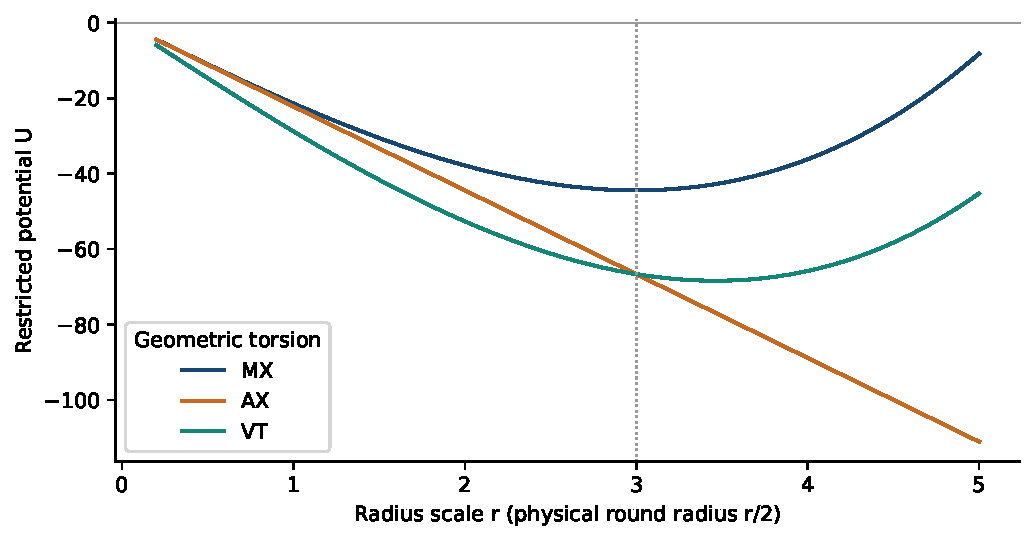
\includegraphics[width=0.93\linewidth]{figures/v3/fig01_radius.pdf}
\caption{Radius potentials at $L=\kappa=1$, with each active torsion coefficient set to one. The MX minimum is $r=3$; the VT minimum is $r=\sqrt{12}$; the AX curve is linear.}\label{fig:fig01_radius}
\end{figure}

The torsion coordinates have positive diagonal static curvature. Their coupling to radius is background dependent:

\begin{equation}\tag{S3}\label{eq:S3}
\begin{aligned}
U_{\eta\eta}&=\frac{3\pi^2Lr}{2\kappa^2},&
U_{VV}&=\frac{\pi^2Lr^3}{6\kappa^2},&
U_{\eta V}&=0,\\
U_{r\eta}&=\frac{3\pi^2L\eta}{2\kappa^2},&
U_{rV}&=\frac{\pi^2Lr^2V}{2\kappa^2}.
\end{aligned}
\end{equation}

Consequently $V$ separates quadratically from $(r,\eta)$ at an AX point with $V=0$, whereas it couples to $r$ in VT and MX. The equality $U_{\eta\eta}=U_{VV}$ at $r=3$ is an equality in these coordinates, not a degeneracy enforced by $SO(3)$. Including $L$ gives further scalar cross terms. Appendix F gives the full gradient and Hessian in one common coordinate system.

\begin{figure}[htbp]
\centering
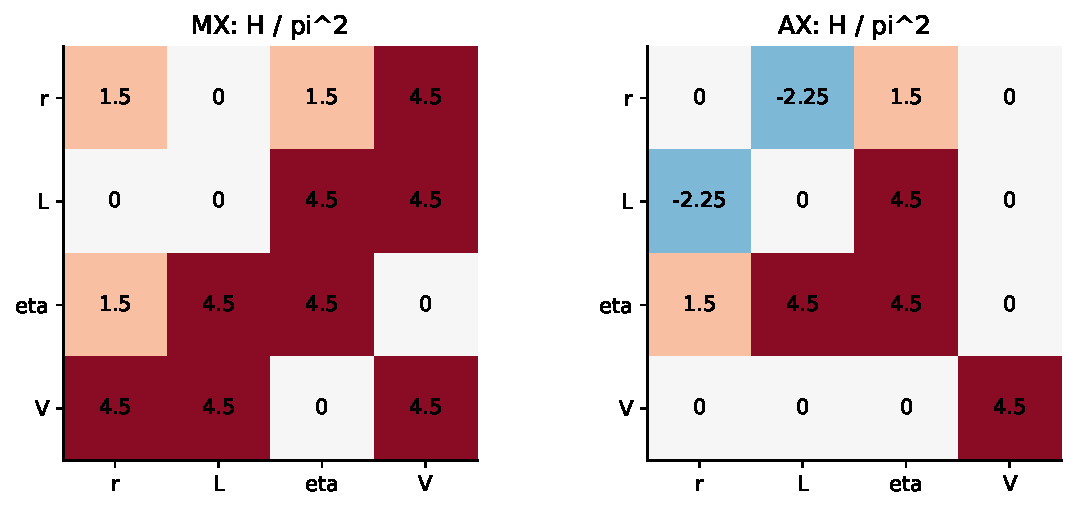
\includegraphics[width=0.93\linewidth]{figures/v3/fig02_scalar.pdf}
\caption{Scalar Hessians in the common coordinates $(r,L,\eta,V)$, divided by $\pi^2$, at the MX point $(3,1,1,1)$ and the AX point $(3,1,1,0)$, with $\kappa=1$. They display couplings between scalar deformations.}\label{fig:fig02_scalar}
\end{figure}

\subsection{Exact scalar action along the circle}

Allow smooth periodic $r(y),L(y),\eta(y),V(y)$, with $r,L>0$, on the round zero-twist coframe. Including the connection derivatives and integrating the total derivatives over the circle gives

\begin{equation}\tag{S4}\label{eq:S4}
\mathcal S_{\mathrm{scalar}}=
\int_0^1dy\left[U_0(r,L,\eta,V)
-\frac{3\pi^2}{4\kappa^2}\frac{r(r')^2}{L}\right].
\end{equation}

Appendix A derives this formula directly from Cartan curvature. Radius carries a circle-derivative term. The $\eta'$ and $V'$ contributions to curvature combine into total derivatives, and no independent $L'$ term remains in the bulk. Here $L(y)$ is the local lapse, while $\int_0^1 L(y)\,dy$ is the circle circumference. Its variation must be specified separately from fixing that circumference. The negative radial derivative coefficient characterizes radial variations of the Euclidean action defined here. The role of lapse and constraints in a canonical formulation is reviewed in \cite{ADM}.

The scalar sector therefore supplies a useful hierarchy: the radius potential at fixed controls, the static response to changing those controls, and the circle-dependent restricted action. For example, the MX radius minimum fixes one derivative to zero, while the remaining scalar gradients need not vanish. This is sufficient for a conditional radius classification and preserves the different roles of size, torsion and circle scale.

In the joint action, scalar changes can couple to shape and twist derivatives through the induced metric (M4). The vanishing of these cross terms in (S4) follows from its round, zero-twist restriction. At nonzero twist the lapse is $\mathcal N$, which differs from the coframe coefficient $L$; an $L'$ cross term in those coordinates need not represent an independent lapse degree of freedom.

%==============================================================================
% Section 4: Spin-2 Sector: Full Shear Completion and Geometric Phase Structure
%==============================================================================
\section{Spin-2 Sector: Full Shear Completion and Geometric Phase Structure}
\label{sec:spin2}

This section completes the squash/shear deformations as the full shear tensor
and presents the final phase diagram of the spin-2 quintet.  The conclusions are:
five-fold degeneracy at the isotropic point; softening of the $m=0$ singlet on
the positive-$\varepsilon$ side; and a second-order phase transition of the
$m=\pm 2$ sector on the negative-$\varepsilon$ side.

\subsection{Full Shear Tensor as the Spin-2 Quintet}

A description in terms of raw geometric variables $(\varepsilon,s,\phi)$ is
useful for following a particular slice but insufficient to represent the entire
spin-2 sector.  We adopt
\begin{equation}
  h_{ij} = \sum_{A=1}^5 q_A\,(T_A)_{ij}
\end{equation}
and treat the five components of $\Sym_0^2(\mathbb{R}^3)$ as a complete spin-2
quintet.  Here $q_A$ are the final variables aligned with the $SO(3)$ irreducible
basis; $\varepsilon$ and $s$ are used as projections of $q_A$ onto specific
directions.

\begin{figure}[H]
  \centering
  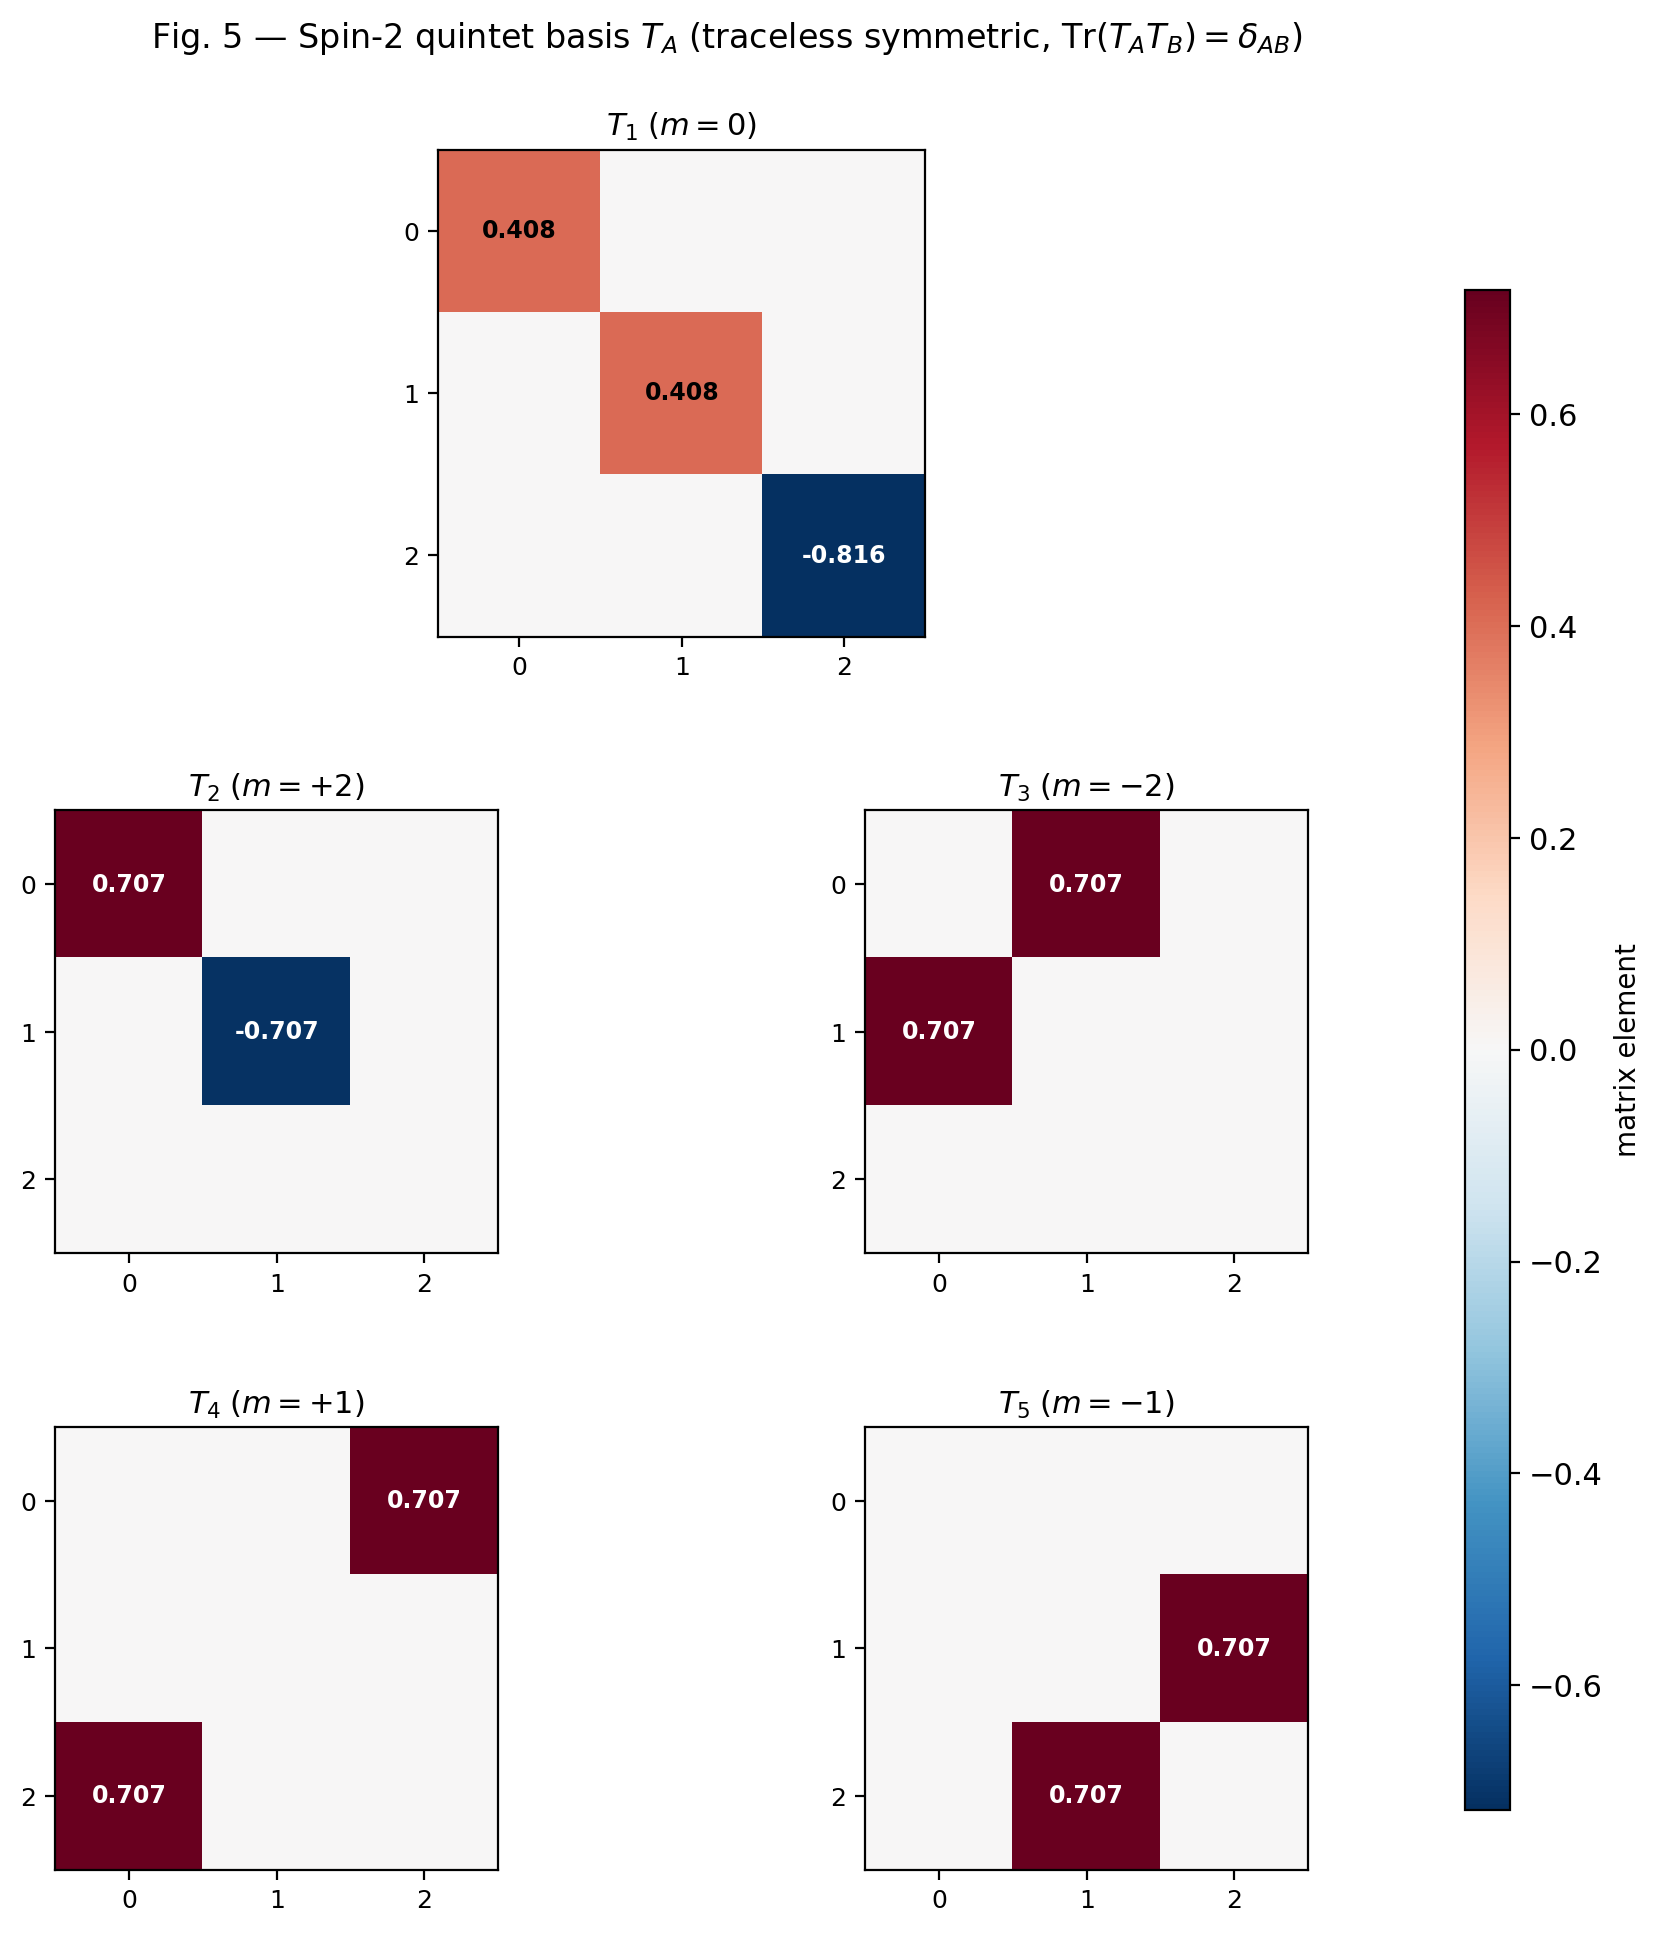
\includegraphics[width=0.72\textwidth]{figures/fig05_TA_basis.png}
  \caption{Basis vectors $T_1,\ldots,T_5$ of the spin-2 quintet
           $\Sym_0^2(\mathbb{R}^3)$.  The three sectors correspond to the
           residual $SO(2)$ representations $m=0$, $m=\pm 2$, and $m=\pm 1$.}
  \label{fig:TA_basis}
\end{figure}

\subsection{Isotropic Point and Schur Degeneracy}

At the isotropic point the residual symmetry is the full $SO(3)$, so the spin-2
Hessian is proportional to the identity matrix on each irreducible representation.
Consequently,
\begin{equation}
  \Veff = V_0 + \lambda\,\tr(h^2) + O(|q|^3)
        = V_0 + \lambda\sum_{A=1}^5 q_A^2 + O(|q|^3),
\end{equation}
giving
\begin{equation}
  H_{AB} = \left.\frac{\partial^2 V}{\partial q_A \partial q_B}\right|_0
          = 2\lambda\,\delta_{AB}.
\end{equation}
The generalised mass is equal for all five components:
\begin{equation}
  \mu_q^2 = 48\pi^2.
\end{equation}
This is the spin-2 sector's Schur degeneracy.

\begin{figure}[H]
  \centering
  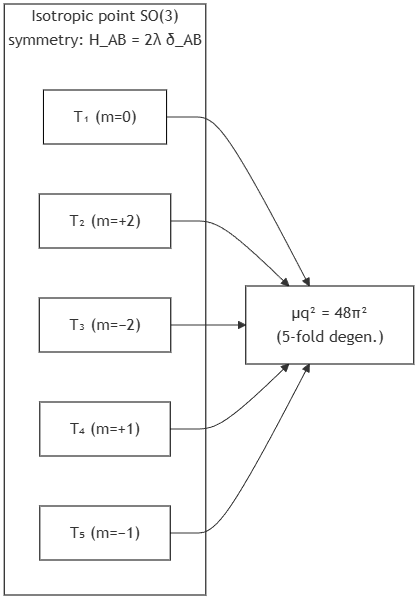
\includegraphics[width=0.6\textwidth]{figures/fig06_five-fold_degeneracy.png}
  \caption{Five-fold degeneracy of the spin-2 quintet at the isotropic point.
           Schur's lemma $H_{AB}=2\lambda\delta_{AB}$ enforces equal mass
           $\mu_q^2=48\pi^2$ for all five components.}
  \label{fig:schur}
\end{figure}

\subsection{$SO(3)$ to $SO(2)$ Splitting under Squash Background}

Under a positive-$\varepsilon$ squash background the symmetry reduces to
$SO(3)\to SO(2)$, and the spin-2 quintet splits as follows.

\begin{table}[H]
\centering
\begin{tabular}{lll}
\toprule
Residual charge & Basis & Interpretation \\
\midrule
$m=0$     & $T_1$          & squash singlet \\
$m=\pm 2$ & $(T_2, T_3)$   & in-plane doublet \\
$m=\pm 1$ & $(T_4, T_5)$   & off-axis doublet \\
\bottomrule
\end{tabular}
\caption{Residual $SO(2)$ decomposition of the spin-2 quintet under a
         positive-$\varepsilon$ squash background.}
\label{tab:SO2split}
\end{table}

The key observation is that the order in which soft modes appear is organised by
these residual representations.

\begin{figure}[H]
  \centering
  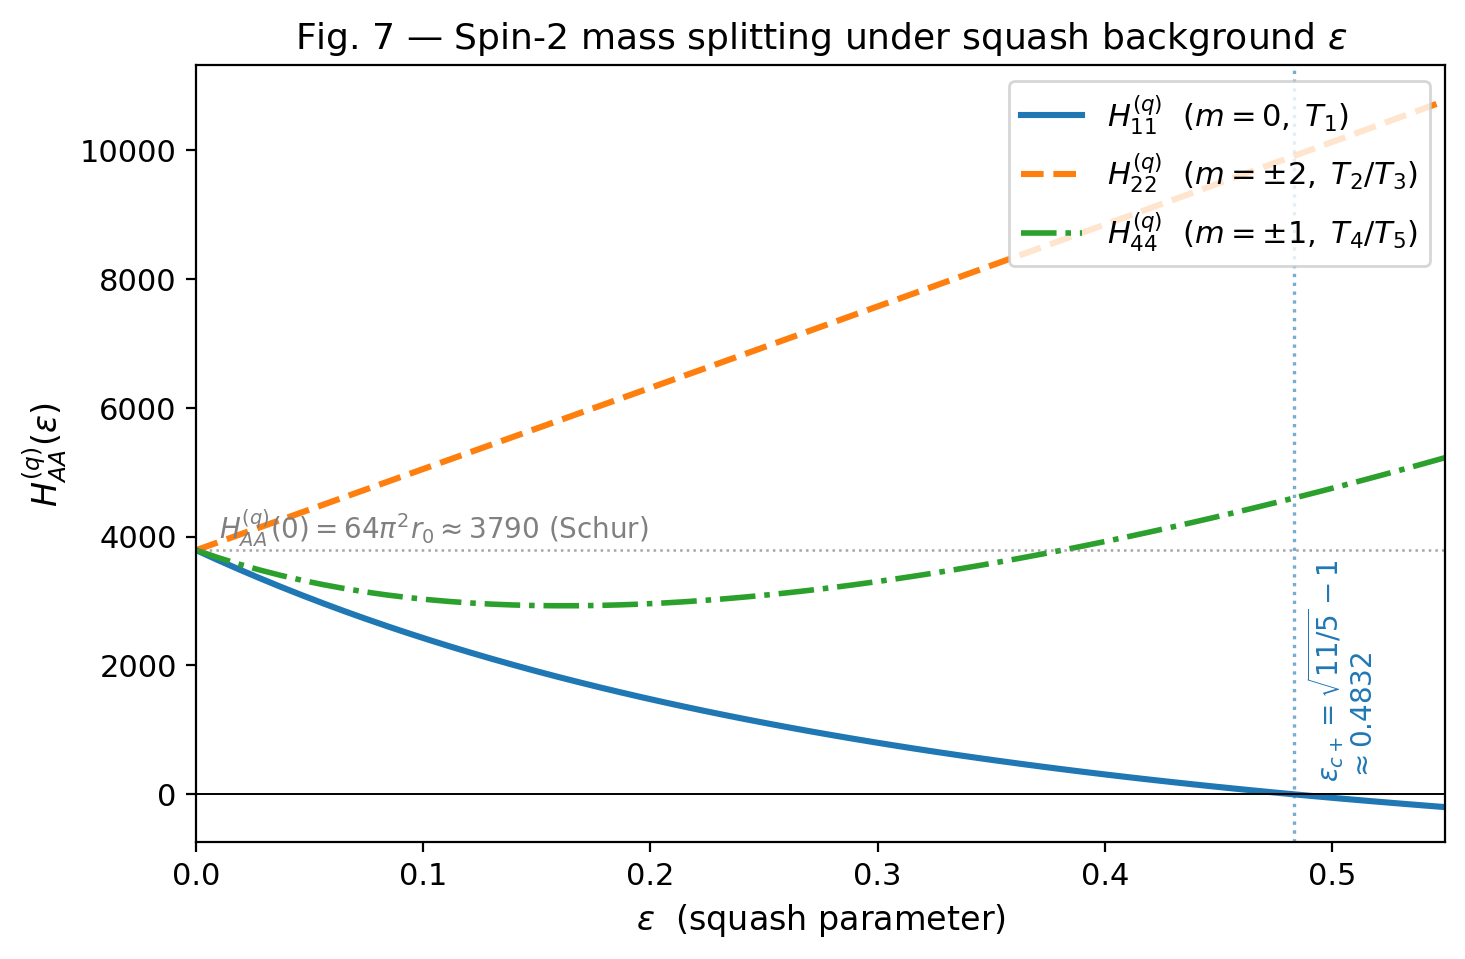
\includegraphics[width=0.75\textwidth]{figures/fig07_spin2_splitting.png}
  \caption{Mass splitting of the spin-2 quintet as a function of the squash
           parameter $\varepsilon$.  The three branches correspond to $m=0$
           (singlet $T_1$), $m=\pm 2$ (doublet $T_2,T_3$), and $m=\pm 1$
           (doublet $T_4,T_5$).  The $m=0$ branch reaches zero first at
           $\varepsilon_{c+}$.}
  \label{fig:spin2_split}
\end{figure}

\subsection{Positive-$\varepsilon$ Side: First Soft Mode}

From the full shear analysis, on the positive side the $T_1$ singlet becomes
soft first.  The critical value is
\begin{equation}
  \varepsilon_{c+} = \sqrt{\frac{11}{5}} - 1 \approx 0.48324,
  \qquad
  r_0(\varepsilon_{c+}) \approx 2.8114,
\end{equation}
at which $\mu_\varepsilon^2\to 0$.

\begin{figure}[H]
  \centering
  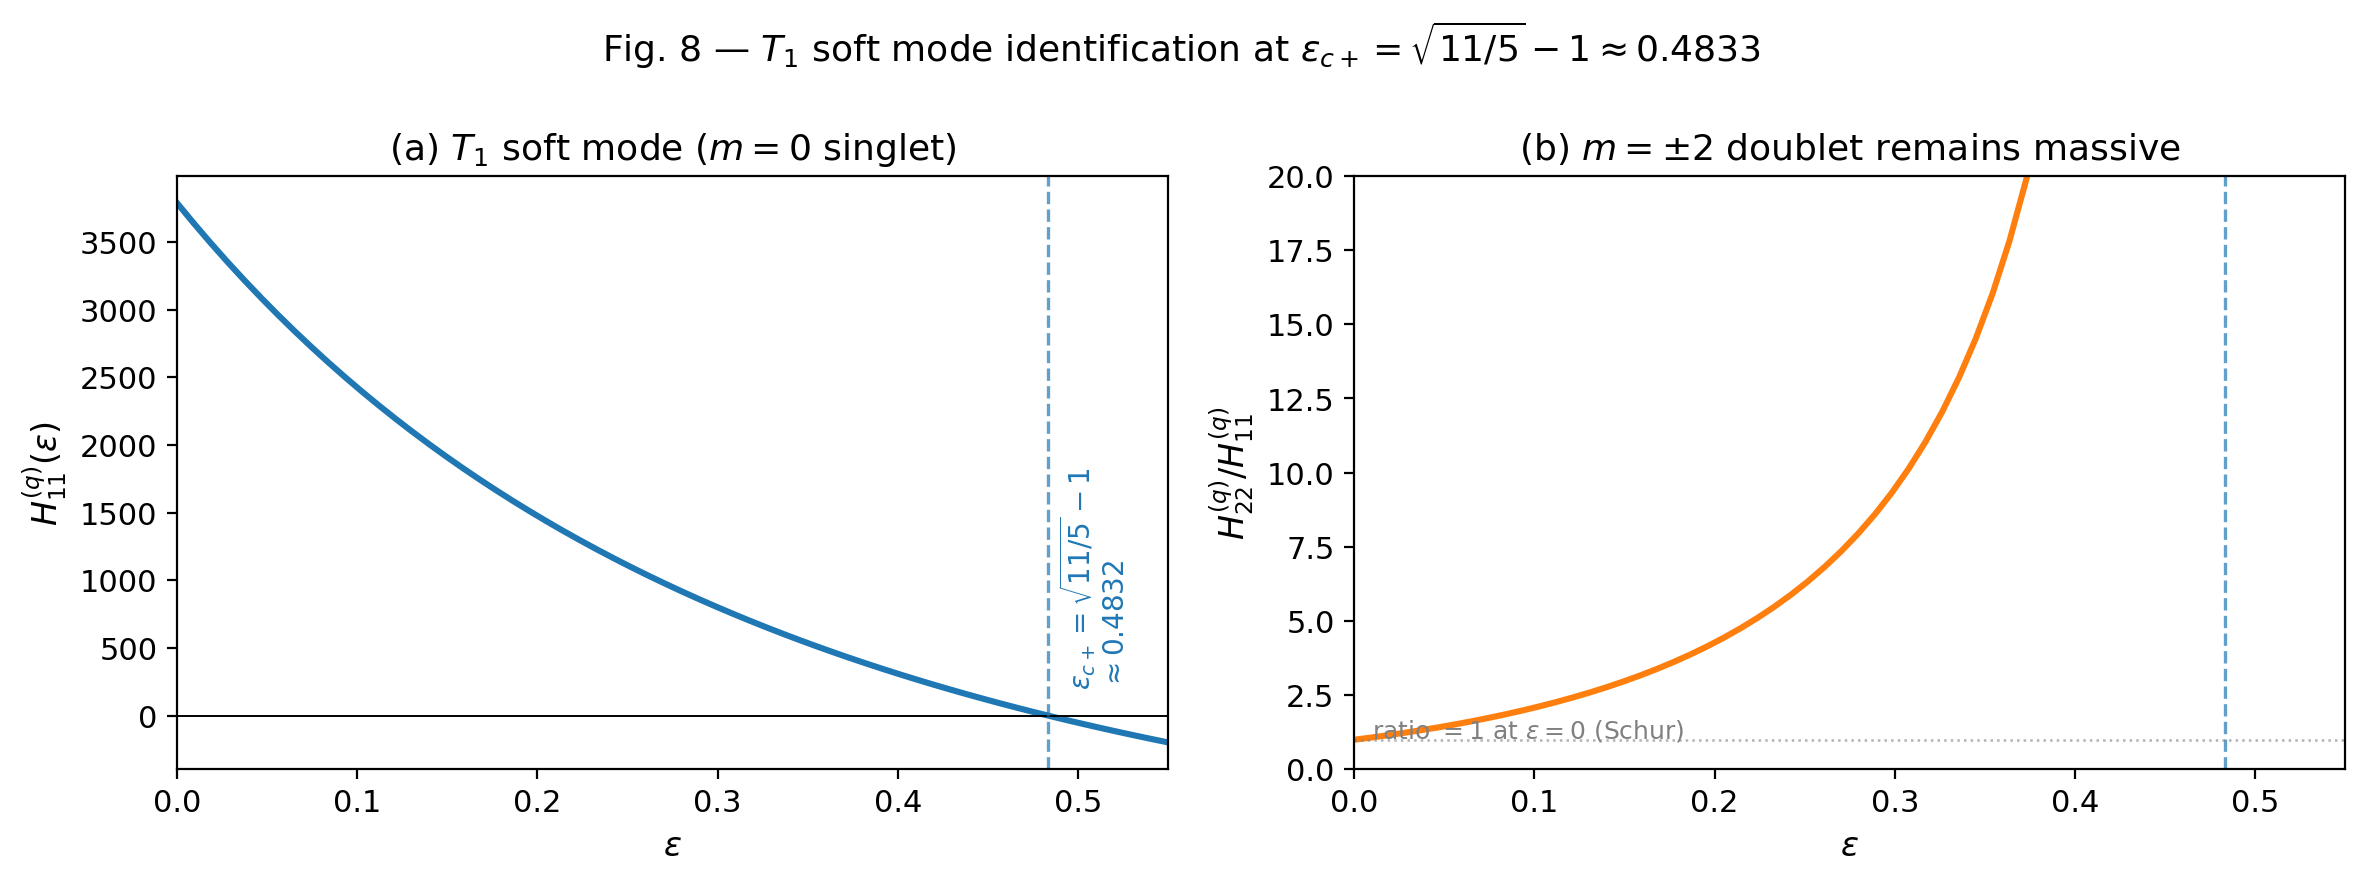
\includegraphics[width=0.85\textwidth]{figures/fig08_soft_mode.png}
  \caption{Softening of the $m=0$ mode $\mu_\varepsilon^2(\varepsilon)$ on the
           positive-$\varepsilon$ side.  The curve reaches zero at the exact
           critical point $\varepsilon_{c+}=\sqrt{11/5}-1\approx 0.483$, while
           the $m=\pm 2$ branch remains massive.}
  \label{fig:soft_mode}
\end{figure}

Key points to emphasise:
\begin{itemize}
  \item The first soft mode is the $m=0$ singlet $T_1$.
  \item The $m=\pm 2$ doublet $(T_2,T_3)$ remains massive even at
        $\varepsilon_{c+}$.
  \item A global scan over $(r,\varepsilon)$ revealed no new global minimum; no
        condensation was found on the axisymmetric slice.
\end{itemize}
Therefore $\varepsilon_{c+}$ is a \emph{softening threshold} on the positive
side rather than the birth point of a fully condensed phase.

\subsection{Negative-$\varepsilon$ Side: $s\neq 0$ Phase Transition}

On the negative side the situation differs.  A three-indicator analysis,
\begin{equation}
  a(\varepsilon) = \frac{d^2 F}{ds^2}\bigg|_{s=0},
  \qquad
  s_0(\varepsilon) = \operatorname*{arg\,min}_s F(s;\varepsilon),
  \qquad
  \mu_s^2(\varepsilon) = \frac{H_{ss}}{G_{ss}},
\end{equation}
locates the critical point at
\begin{equation}
  \varepsilon_{c-} = \frac{1}{\sqrt{2}} - 1 \approx -0.29309 \pm 0.00019,
\end{equation}
with the three indicators converging to $-0.29303$, $-0.29335$, and $-0.29289$,
respectively.  The closed-form exact value $1/\!\sqrt{2}-1$ agrees with the
numerical estimate and is derived directly from the condition $H_{22}^q=0$ (see
Appendix~\ref{app:D}).

For the Landau free energy
\begin{equation}
  F(s;\varepsilon) = a(\varepsilon)\,s^2 + b(\varepsilon)\,s^4 + O(s^6),
\end{equation}
one finds $b(\varepsilon)\in[2288,7805]>0$ near the critical point, confirming a
\emph{second-order transition}.  The order-parameter fit gives
\begin{equation}
  s_0 \propto |\varepsilon - \varepsilon_c|^\beta,
  \qquad
  \beta = 0.4678,\quad R^2 = 0.987,
\end{equation}
consistent with a mean-field-like continuous transition.  $\beta$ falls slightly
below the mean-field value $1/2$ by $1/2 - \beta \approx 0.032$; the precise
physical meaning of this deviation---which is sensitive to the finite-range fit,
higher-order terms, and the finite precision of the minisuperspace Landau
description---is beyond the scope of this paper.

\begin{figure}[H]
  \centering
  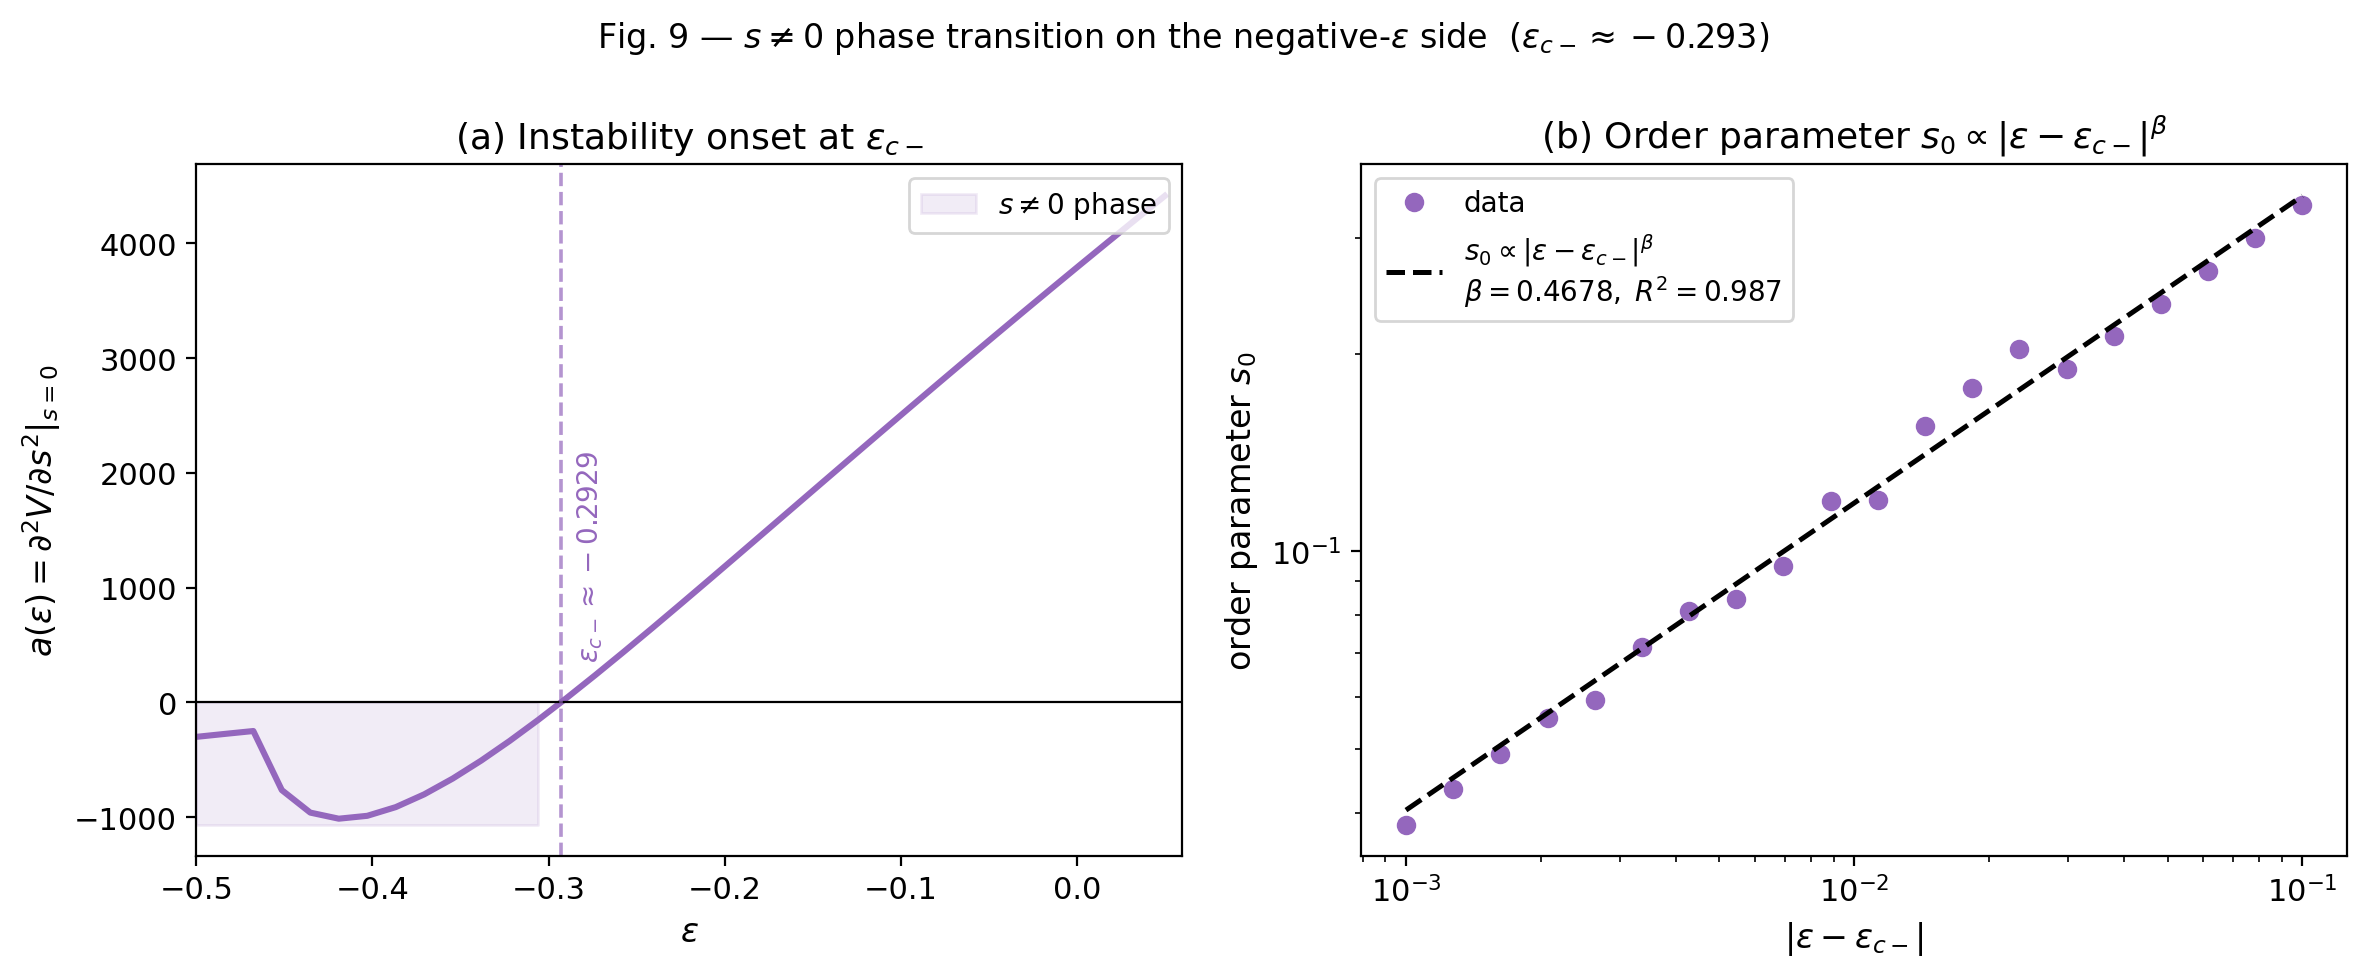
\includegraphics[width=0.85\textwidth]{figures/fig09_sneg_phase.png}
  \caption{Phase structure on the negative-$\varepsilon$ side.  The order
           parameter $s_0(\varepsilon)$ emerges continuously at
           $\varepsilon_{c-}=1/\!\sqrt{2}-1\approx -0.293$, consistent with a
           second-order transition into the $s\neq 0$ phase.}
  \label{fig:sneg_phase}
\end{figure}

\subsection{Geometric Interpretation}

In the $s\neq 0$ vacuum, $\mu_s^2$ becomes soft near the transition and then
returns to positive values, while $\mu_\varepsilon^2$ remains large and positive
over a wide range.  Furthermore, the $\phi$ direction is a pseudo-Goldstone
rather than an exact Goldstone, reflecting that $SO(2)$ is explicitly broken in
the $s\neq 0$ background.

The final picture of the spin-2 sector is summarised as follows.
\begin{enumerate}
  \item The full shear 5-plet is five-fold degenerate at $\mu_q^2=48\pi^2$ at
        the isotropic point.
  \item The first unstable direction on the positive side is the $m=0$ singlet
        $T_1$.
  \item On the negative side the $m=\pm 2$ sector governs the second-order
        transition into the $s\neq 0$ phase.
\end{enumerate}
This phase diagram plays the central role of the spin-2 block in the Landau-EFT
description of \S\ref{sec:eft}.

\section{Spin-2: shape splitting and continuous bifurcation}

\label{sec:5}

\subsection{The quintet and its axial splitting}

Write $h=q_AT_A$, where $T_A$ is the orthonormal symmetric traceless basis of Appendix C. At $\omega=0$ the scalar controls multiply the shape action by $\mathcal K$ and add a shape-independent constant. At the round point its Hessian is $8\mathcal K\delta_{AB}$, so all five normalized directions have the same positive curvature. For the axial reference $M_0=\mathrm{diag}(a,a,a^{-2})$, with $a=(1+\epsilon)^{1/3}$, $\epsilon>-1$, use the paths $M=M_0e^{q_AT_A}$ one at a time. Their curvatures split into a singlet and two doublets:

\begin{equation}\tag{T1}\label{eq:T1}
\begin{aligned}
H_0&=\frac{8\mathcal K(4-a^6)}{3a^8},\\
H_2&=\frac{8\mathcal K(2a^6-1)}{a^2},\qquad (T_2,T_3),\\
H_1&=\frac{4\mathcal K(a^6+1)}{a^8},\qquad (T_4,T_5).
\end{aligned}
\end{equation}

At $a=1$ these agree with the round value. Residual rotations in the 01 plane rotate $(T_2,T_3)$ with twice the angle and $(T_4,T_5)$ with the angle itself. The specified exponential path fixes the meaning of the second derivatives. Off a stationary shape, another path with the same tangent can have a different second derivative, as derived in Appendix D. In particular, the zero of $H_0$ at $\epsilon=1$ is a curvature zero along that path.

\begin{figure}[htbp]
\centering
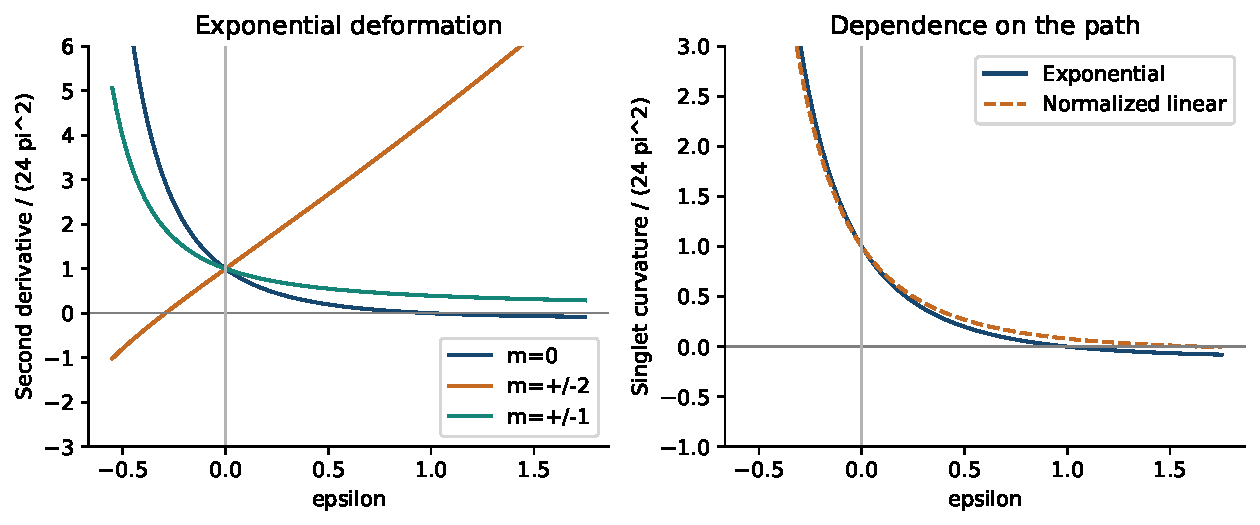
\includegraphics[width=0.93\linewidth]{figures/v3/fig05_shear.pdf}
\caption{The singlet and two doublet curvatures, normalized by $24\pi^2$ at $r=3$, $L=\kappa=1$. The second panel compares two paths with the same tangent at the axial background.}\label{fig:fig05_shear}
\end{figure}

\subsection{Exact doublet minimization at fixed axial control}

Fix $a$ and minimize over the full doublet, $M=M_0\exp(q_2T_2+q_3T_3)$. Let $\rho=(q_2^2+q_3^2)^{1/2}$. The eigenvalues of $S$ are $a^2e^{\sqrt2\rho},a^2e^{-\sqrt2\rho},a^{-4}$. Thus $z=2\cosh(\sqrt2\rho)\ge2$ reduces the problem to a convex quadratic:

\begin{equation}\tag{T2}\label{eq:T2}
F(a,z)=a^4(z^2-4)-2a^{-2}z+a^{-8}
=a^4(z-a^{-6})^2-4a^4.
\end{equation}

\begin{equation}\tag{T3}\label{eq:T3}
\begin{aligned}
\rho_{\ast}(a)&=
\begin{cases}
0,&a^6\ge1/2,\\
\mathrm{arcosh}(1/(2a^6))/\sqrt2,&a^6<1/2,
\end{cases}\\
F_{\min}(a)&=
\begin{cases}
a^{-8}-4a^{-2},&a^6\ge1/2,\\
-4a^4,&a^6<1/2.
\end{cases}
\end{aligned}
\end{equation}

The critical control is $\epsilon_c=1/\sqrt2-1$. For $\epsilon<\epsilon_c$ the minimum has three unequal shape eigenvalues; it approaches the axial shape continuously at the boundary. More precisely,

\begin{equation}\tag{T4}\label{eq:T4}
\begin{aligned}
\rho_{\ast}&=2^{3/4}\sqrt{\epsilon_c-\epsilon}
+O((\epsilon_c-\epsilon)^{3/2}),\\
[\,\partial_\epsilon^2 F_{\min}\,]_{\mathrm{right}}
-[\,\partial_\epsilon^2 F_{\min}\,]_{\mathrm{left}}
&=32\,2^{1/3}.
\end{aligned}
\end{equation}

Both $F_{\min}$ and its first derivative are continuous at $\epsilon_c$. The quartic coefficient in the local expansion in $\rho$ is $2\,2^{1/3}>0$ at criticality. These facts characterize a continuous bifurcation of constrained shape minima, or a continuous shape transition within this finite-dimensional minimization problem.

\begin{figure}[htbp]
\centering
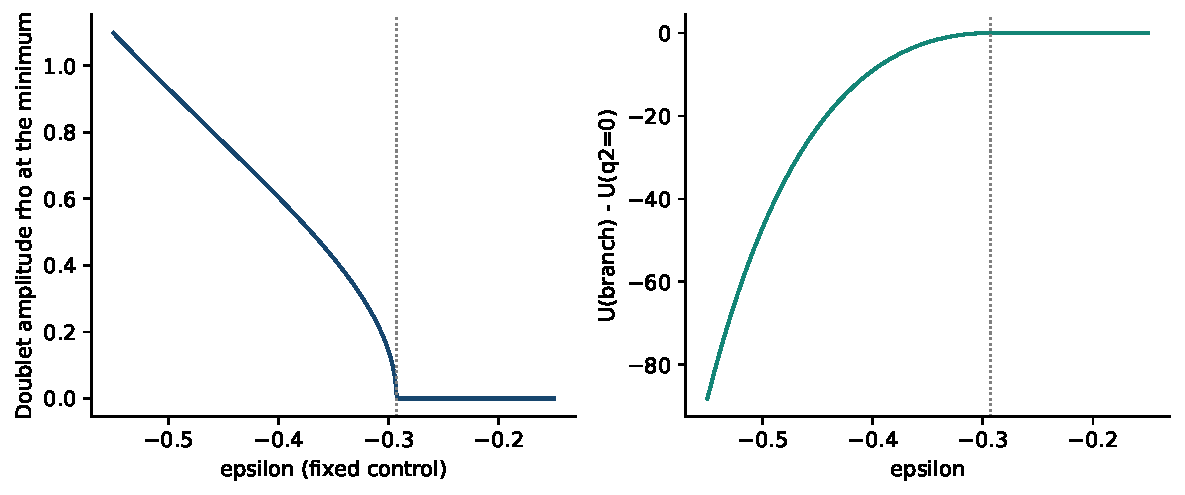
\includegraphics[width=0.93\linewidth]{figures/v3/fig06_branch.pdf}
\caption{Doublet amplitude and the potential gain at fixed axial control. The dotted line is $\epsilon_c$. For nonzero amplitude the minimizers form a rotation orbit, not two isolated minima.}\label{fig:fig06_branch}
\end{figure}

The two signs of $q_2$ on the cut $q_3=0$ are points on the circle $q_2^2+q_3^2=\rho_{\ast}^2$. Residual $SO(2)$ rotations connect that circle. When shapes related by rotations and axis relabeling are identified, it represents one triaxial shape class at each fixed control.

\subsection{Global minimum of the static shape potential}

At fixed scalar controls and zero twist, every positive-definite $S$ of determinant one has an eigenvalue representation of the form used in (T2), after choosing an axis order. Minimizing (T3) also over $a>0$ therefore covers all shapes, modulo rotations. For $a^6<1/2$, $F_{\min}>-2^{4/3}>-3$. On the complementary branch,

\begin{equation}\tag{T5}\label{eq:T5}
F_{\min}+3=
\frac{(a^2-1)^2(3a^4+2a^2+1)}{a^8}\ge0.
\end{equation}

Equality requires $a=1,z=2$, hence $S=I$. On this zero-twist slice, the round shape is the unique global minimizing shape of the static potential, modulo rotations. Since the twist term in (M3) is nonnegative, minimizing over twist as well gives $\omega=0$. At a prescribed nonzero twist, the shape dependence of the last term in (M3) generally shifts the shape minimum. The fixed-control bifurcation and the full-shape minimum above are complementary results of the static zero-twist potential. At fixed torsion and circle circumference, combining this bound with Section 3 also selects the round radius minimum when $V\ne0$ and $\eta^2<4$.

\begin{figure}[htbp]
\centering
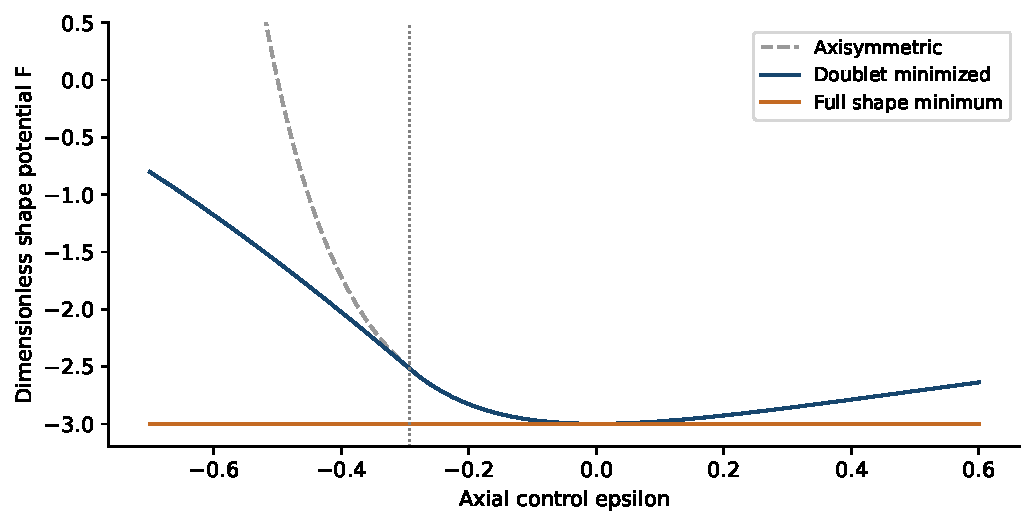
\includegraphics[width=0.93\linewidth]{figures/v3/fig07_shape_minima.pdf}
\caption{The axial shape potential, its doublet-minimized value and the full-shape lower bound $F=-3$. Releasing the axial control selects $\epsilon=0$, $\rho=0$.}\label{fig:fig07_shape_minima}
\end{figure}

\subsection{Circle-dependent shape}

Set $\omega=0$ and write $B=M^{\mathsf T}M$, with $\det B=1$. Then $Y=0$ and $\mathrm{tr}(B^{-1}B')=0$. The derivative part of (M6) becomes

\begin{equation}\tag{T6}\label{eq:T6}
\mathcal L_{\partial}\big|_{\omega=0}
=-\frac{3\pi^2r(r')^2}{4\kappa^2L}
+\frac{\pi^2r^3}{32\kappa^2L}
\mathrm{tr}\!\left[(B^{-1}B')^2\right].
\end{equation}

The shape term is nonnegative: $B^{-1}B'$ is similar to the symmetric matrix $B^{-1/2}B'B^{-1/2}$. Near a constant round reference, $M=e^h$ gives the quadratic coefficient $\pi^2r_0^3\mathrm{tr}[(h')^2]/(8\kappa^2L_0)$. The scalar--shape derivative cross term vanishes exactly at zero twist. Thus the static bifurcation and a positive shape derivative cost can be described in the same sector. Their extension to nonzero twist requires the joint terms of Section 6.

%==============================================================================
% Section 6: Unified Geometric Landau EFT
%==============================================================================
\section{Unified Geometric Landau EFT}
\label{sec:eft}

This section consolidates the results of \S\S\ref{sec:pont}--\ref{sec:spin1}
into a single final effective theory.  The key point is that in the final basis
the quadratic sector is block-diagonally organised and the allowed interaction
terms are described transparently by the invariant basis and representation-
theoretic selection rules.

\subsection{Raw Quadratic Data}

In the raw basis the effective potential is
\begin{equation}
\begin{aligned}
  \Veff &= V_0
    + \tfrac{1}{2}\mu_q^2\,\tr(h^2)
    + \tfrac{1}{2}\mu_\omega^2|\omega|^2
    + \tfrac{1}{2}\mu_\delta^2|\delta|^2
    + m_{\omega\delta}\,\omega\cdot\delta \\
    &\quad + c_\omega\,h_{ij}\omega_i\omega_j
    + c_\delta\,h_{ij}\delta_i\delta_j
    + O(4),
\end{aligned}
\end{equation}
where
\begin{equation}
  \mu_q^2 = 48\pi^2,
  \quad
  \mu_\omega^2 = 52.6379,
  \quad
  \mu_\delta^2 = 3789.9295,
  \quad
  m_{\omega\delta} = -631.6544,
\end{equation}
\begin{equation}
  c_\omega = 105.28,
  \qquad
  c_\delta = 1894.96,
  \qquad
  c_{\omega\delta} = 0 \quad\text{(at the isotropic point)}.
\end{equation}
The raw geometric description is necessary for tracing the geometrical origins but
is redundant as an organiser of physical degrees of freedom.  The final basis is
derived via the physical/auxiliary decomposition of \S\ref{sec:spin1}.

\subsection{Final Quadratic EFT}
\label{sec:eft:quad}

In the final basis the quadratic sector decomposes conceptually as
\begin{equation}
  \mathcal{L}_\mathrm{quad}
  = \mathcal{L}_r
  + \mathcal{L}_{q_A}
  + \mathcal{L}_X
  + \mathcal{L}_Y
  + \mathcal{L}_{\eta,V},
\end{equation}
with
\begin{equation}
  \mathcal{L}_{q_A} = -\frac{1}{2}\mu_q^2 \sum_{A=1}^5 q_A^2,
  \qquad
  \mathcal{L}_X = \frac{1}{2}\dot{X}^T G_\phys \dot{X} - \frac{1}{2} X^T H_\phys X,
  \qquad
  \mathcal{L}_Y = -\frac{1}{2} Y^T H_\mathrm{null} Y.
\end{equation}

Since all 21 mixed Hessian components between $X_k$ and $(q_A,r,\eta)$ vanish,
quadratic decoupling of the spin-1 sector is an exact statement in the final
basis.  All 10 spin-2--torsion cross-Hessian components also vanish at the
isotropic point, and the radial--$V$ cross-Hessian is zero as well.  However,
the radial--$\eta$ cross-Hessian is non-zero ($\approx 118.4$), so the
scalar/torsion subsector forms a coupled $(r,\eta)$ block with $V$ remaining
independent.  Thus the natural block decomposition at quadratic order is
\begin{equation}
  (q_A)\;\oplus\;(X_k)\;\oplus\;(Y_k)\;\oplus\;
  \bigl[(r,\eta)\;\text{block}\;\oplus\;(V)\bigr].
\end{equation}

\begin{figure}[H]
  \centering
  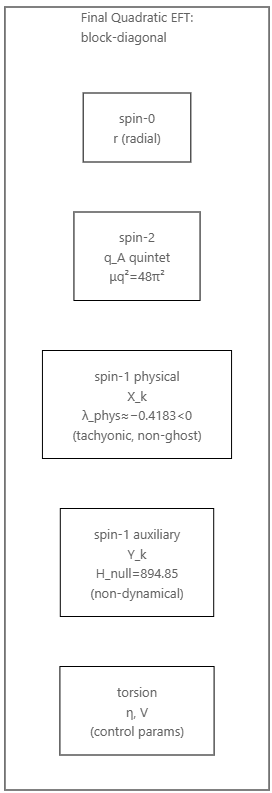
\includegraphics[width=0.4\linewidth]{figures/fig13_final_quadratic_sector.png}
  \caption{Quadratic block organisation of the final sector.  The spin-1 sector
           fully decouples; the spin-2 sector decouples from torsion; the
           scalar/torsion subsector contains a coupled $(r,\eta)$ block.}
  \label{fig:quadratic_block}
\end{figure}

\subsection{Invariant Basis and Selection Rules}

The low-order scalars of the Landau-EFT are organised by the invariant basis
\begin{equation}
  I_2 = \tr(h^2),
  \qquad
  I_3 = h_{ij}\omega_i\omega_j,
  \qquad
  I_4 = \tr(h^3),
  \qquad
  W_2 = \omega_i\omega_i.
\end{equation}
An exact check confirms $I_3 = q_A F_A(\omega)$ in the final $T_A$ basis.  At
quartic order the natural helper invariants are $I_2^2$, $I_2 W_2$, $W_2^2$.

This organisation implies:
\begin{itemize}
  \item Representative allowed cubic terms are $h_{ij}\omega_i\omega_j$ and
        $h_{ij}\delta_i\delta_j$.
  \item Quadratic cross-terms in $X_k$ vanish in the final basis.
  \item Known forbidden terms $H_\mathrm{sym}$ and $K_\mathrm{sym}$ are excluded
        by the representation-theoretic selection rule.
\end{itemize}

\begin{figure}[H]
  \centering
  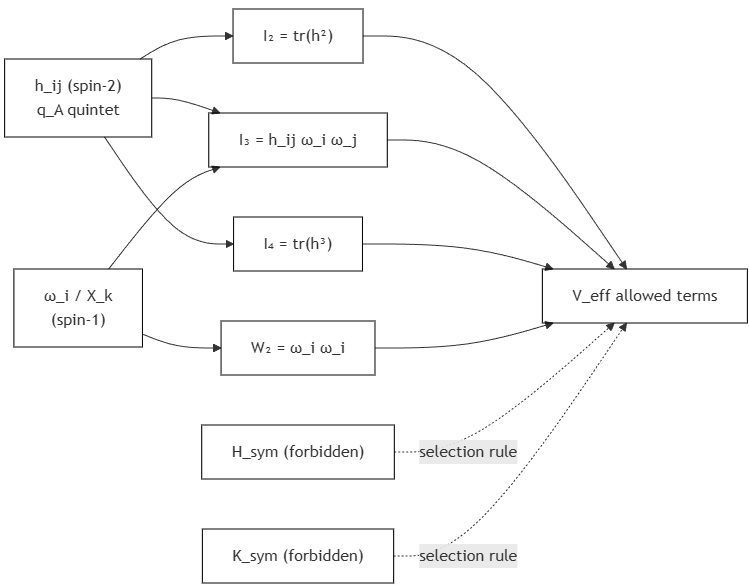
\includegraphics[width=0.75\textwidth]{figures/fig14_EFT_connection_structure.png}
  \caption{Connection structure of low-order invariants in the Landau-EFT.
           Solid arrows indicate allowed terms; dashed arrows indicate terms
           forbidden by selection rules.}
  \label{fig:EFT_conn}
\end{figure}

\subsection{Final Mode Dictionary}
\label{sec:eft:dict}

We recapitulate the mode dictionary adopted in this paper.

\begin{table}[H]
\centering
\begin{tabularx}{\textwidth}{l l l X}
\toprule
Variable & Final classification & Role & Comment \\
\midrule
$r$   & spin-0 & isotropic radius & equilibrium $r_0=3$ \\
$q_A$ & spin-2 & full shear quintet & $\mu_q^2=48\pi^2$ \\
$X_k$ & spin-1 physical  & propagating mixed mode & quadratic decoupled \\
$Y_k$ & spin-1 auxiliary & non-propagating auxiliary & not gauge \\
$\eta$ & spin-0 torsion & AX parameter & input/control \\
$V$   & spin-0 torsion & VT parameter & input/control \\
\bottomrule
\end{tabularx}
\caption{Final mode dictionary.  The raw geometric variables $(\omega_i,\delta_i)$
         are an intermediate description; they are translated to $X_k$ and $Y_k$
         in the final physical dictionary.}
\label{tab:mode_dict}
\end{table}

The block decomposition of the quadratic sector is as given in \S\ref{sec:eft:quad}:
the spin-1 and spin-2 sectors decouple, while the scalar/torsion subsector
retains the coupled $(r,\eta)$ block identified there.

\begin{figure}[H]
  \centering
  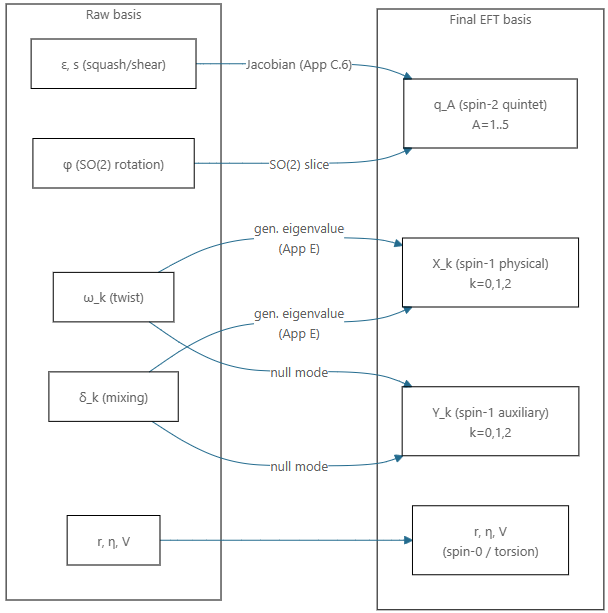
\includegraphics[width=0.85\textwidth]{figures/fig15_assignment_raw2final.png}
  \caption{Overall transformation from raw geometric variables to the final EFT
           basis.  Arrows indicate the assignment of each variable.}
  \label{fig:raw2final}
\end{figure}

\subsection{Interpretation as a Geometric Landau EFT}

From the above results the model can be understood not merely as a description of
a numerical potential in the gravitational minisuperspace, but as a finite-
degree-of-freedom \emph{geometric Landau-EFT}:
\begin{enumerate}
  \item Order-parameter-like geometric degrees of freedom are organised by
        irreducible representations.
  \item The quadratic sector is block-organised into representation-theoretic
        blocks.  The spin-1 sector fully decouples; the scalar/torsion side has
        the refined block structure~--- a coupled $(r,\eta)$ block and an
        independent $V$ direction.
  \item Allowed interactions are described by the invariant basis and
        representation-theoretic selection rules.
\end{enumerate}
This section thus translates the behaviour of the geometric degrees of freedom in
the $\Sthree\times\Sone$ topology of the minisuperspace reduction into a unified
theoretical language.

The cross-Hessian analysis of \S\ref{sec:eft:quad} shows that this block
organisation is exact at quadratic order (see also Appendix~\ref{app:H:numerical}
for the full numerical tables).  In addition, the torsion block $H^{(\eta,V)}$ at
the isotropic point is diagonal and doubly degenerate with positive eigenvalues
($\approx 355.3$), while the coupled $(r,\eta)$ $2\times 2$ block becomes
saddle-point-type (indefinite) in the AX mode, reflecting the flat-direction
nature of $r$, yielding $\lambda_\mathrm{min}<0$.

%==============================================================================
% Section 7: Physical Interpretation and Outlook
%==============================================================================
\section{Physical Interpretation and Outlook}
\label{sec:discussion}

This section clarifies what has been completed and what has not yet been
settled.

\subsection{What Has Been Completed in homogeneous bulk geometric sector}

The principal items established in this paper at the classical quadratic level
of the homogeneous minisuperspace geometric sector are summarised in
\S\ref{sec:conclusion}.  Here we add a remark on the scope limitation.

``Quadratic block organisation'' means that the homogeneous bulk sector can be
decomposed into spin-2, physical spin-1, auxiliary spin-1, and scalar/torsion
subsectors.  Note, however, that the scalar/torsion subsector is not fully
diagonal in the $(r,\eta,V)$ variables: at quadratic order the radial mode mixes
with axial torsion, while the $V$ direction remains separate at the isotropic
point.

It is important to emphasise that \emph{inhomogeneous modes are not addressed
here}.  This paper concerns the classical EFT structure of the homogeneous bulk
geometric sector.

\subsection{What Is Not Claimed Here}

The following claims are deliberately withheld.
\begin{itemize}
  \item Full stability including inhomogeneous modes beyond minisuperspace.
  \item Identification of the generalised eigenvalue $\lambda_\phys$ with a
        universal mass squared.
  \item A claim that the full 4-dimensional deformed geometry constitutes a new
        Lie group manifold.
  \item Complete action generation including arbitrary non-invariant polynomials.
\end{itemize}
These are not in contradiction with the results of this paper; they are
consciously outside the stated scope.

\subsection{Relation to the Thermal Interpretation of the $S^1$ Direction}

Since paper~I \cite{paper1}, the $\Sone$ direction has been regarded as a natural
connection point to a thermal interpretation.  Although this paper does not
explicitly discuss that connection, the final-basis organisation of the homogeneous
geometric sector provides a firmer foundation for future discussions of:
\begin{itemize}
  \item the stable sector of the background geometry;
  \item control parameters coupled to thermal deformations;
  \item the separation of bulk geometric response from thermally dependent
        responses.
\end{itemize}

\subsection{Toward Future Extensions}

The future tasks for this model are the following.
\begin{enumerate}
  \item Introduction of inhomogeneous fluctuations including local degrees of
        freedom.
  \item Settings involving boundaries and interfaces.
  \item Connection between homogeneous bulk modes and localised modes.
  \item Bridges to physical observables including thermal and Lorentzian
        interpretations.
\end{enumerate}

%==============================================================================
% Section 8: Conclusion
%==============================================================================
\section{Conclusion}
\label{sec:conclusion}

We have reorganised the homogeneous $\Sthree\times\Sone$ minisuperspace geometry
of Einstein--Cartan + Nieh--Yan theory along the final irreducible basis.  As a
result, the following five structures close as a single theoretical framework:
\begin{itemize}
  \item Pontryagin protection in the AX/VT torsion modes,
  \item completion of the spin-2 quintet by the full shear tensor,
  \item physical/auxiliary decomposition of the twist-mixing system,
  \item quadratic decoupling in the final basis, and
  \item a unified geometric Landau-EFT in the invariant basis.
\end{itemize}

In particular, the central message of this paper can be distilled into one
sentence:
\begin{quote}
  \itshape
  The homogeneous geometric sector of the minisuperspace is a completed
  geometric Landau-EFT, organised along the spin-0/1/2 irreducible
  representations.
\end{quote}

From this conclusion, the present model establishes one closed framework for the
classical homogeneous geometric sector.  On the other hand, the next challenges
--- thermal interpretation, local degrees of freedom, and interface analysis ---
are left to future work.  This paper provides the theoretical junction that
delineates those branches.

\Needspace{19\baselineskip}
\section*{Acknowledgments}
The author acknowledges the use of the following AI tools during manuscript
preparation: Claude Opus~4.6 (Anthropic; accessed 2026-03),
Gemini~3.1 Pro (Google; accessed 2026-03), Grok 4.2 (xAI; accessed 2026-03),
and GPT-5.4 Thinking via ChatGPT (OpenAI; accessed 2026-03).
These tools were used for language editing (including Japanese--English
translation), outlining and improving exposition, drafting and reviewing
auxiliary code (scripts and pseudocode) that was subsequently tested and
validated by the author, and proposing candidate consistency checks and
alternative derivations to be independently verified by the author.

The AI tools did not determine the scientific claims of this work; numerical
results and figures were produced by deterministic calculations of the stated
formulas, rather than by generative image synthesis.  The author
takes full responsibility for the content and for any remaining errors.

For this revision, Codex (OpenAI; accessed 2026-11) also assisted with
computational and plotting code, bilingual presentation, and symbolic and
numerical checks.

This work was developed within the informal collaborative project
\textbf{DPPU} (\textbf{D}onut-like topology, \textbf{P}lanck-scale
compactness, \textbf{P}recession dynamics, \textbf{U}niverse).

\appendix
\section{Cartan connection and the scalar circle action}

\label{app:A}

Use $de^a=\tfrac12 C^a{}_{bc}e^b\wedge e^c$ and $\Gamma^a{}_b=\Gamma^a{}_{bc}e^c$. Metric compatibility and the specified geometric torsion give

\begin{equation}\tag{A1}\label{eq:A1}
\begin{aligned}
\Gamma^{\mathrm{LC}}_{abc}&=\tfrac12(C_{abc}+C_{cba}-C_{bac}),\\
K_{abc}&=-\tfrac12(T_{abc}+T_{bca}-T_{cab}),\qquad
\Gamma^{\mathrm{EC}}=\Gamma^{\mathrm{LC}}+K,\\
R^a{}_{bcd}&=e_c(\Gamma^a{}_{bd})-e_d(\Gamma^a{}_{bc})
+\Gamma^a{}_{ec}\Gamma^e{}_{bd}-\Gamma^a{}_{ed}\Gamma^e{}_{bc}
+\Gamma^a{}_{be}C^e{}_{cd}.
\end{aligned}
\end{equation}

Substitution verifies $C^a{}_{bc}+\Gamma^a{}_{cb}-\Gamma^a{}_{bc}=T^a{}_{bc}$. For $e=A(y)\bar e$, with $\bar e=(\sigma^0,\sigma^1,\sigma^2,dy)$, the full exterior derivative is

\begin{equation}\tag{A2}\label{eq:A2}
\begin{aligned}
C^a{}_{bc}
&=A^a{}_d(A^{-1})^e{}_b(A^{-1})^f{}_c\bar C^d{}_{ef}\\
&\quad +(\partial_y A^a{}_f)
\left[(A^{-1})^3{}_b(A^{-1})^f{}_c
-(A^{-1})^3{}_c(A^{-1})^f{}_b\right],\\
e_c(\Gamma^a{}_{bd})&=(A^{-1})^3{}_c\partial_y\Gamma^a{}_{bd}.
\end{aligned}
\end{equation}

For constant $A=O\left(\begin{smallmatrix}rM&0\\L\omega^{\mathsf T}&L\end{smallmatrix}\right)$, these equations reduce to the constant-coframe algebra. With $S=MM^{\mathsf T}$ their scalar contraction is

\begin{equation}\tag{A3}\label{eq:A3}
R=\frac{8}{r^2}\lbrace[\mathrm{tr}S]^2-2\mathrm{tr}(S^2)\rbrace
-\frac{8L^2}{r^4}\lVert M\omega\rVert^2-\frac{6\eta^2}{r^2}-\frac{2V^2}{3}.
\end{equation}

For diagonal $M=\mathrm{diag}(f_0,f_1,f_2)$, $\prod_i f_i=1$, the spatial structure constants are $4f_i^2\epsilon_{ijk}/r$. Their substitution gives the shape term in (A3); the matrix transformation (A2) supplies the general coframe and twist. Multiplying by $-\pi^2Lr^3/(8\kappa^2)$ proves (M3). For the scalar circle family, direct use of (A1)--(A2) instead gives

\begin{equation}\tag{A4}\label{eq:A4}
\begin{aligned}
R_{\mathrm{EC}}
&=\frac{24-6\eta^2}{r^2}-\frac{2V^2}{3}
-\frac{6r''}{L^2r}-\frac{6(r')^2}{L^2r^2}
+\frac{6r'L'}{L^3r}
+\frac{2}{L}\left(V'+\frac{3r'V}{r}\right),\\
N&=-\frac{6}{Lr^3}\partial_y(\eta r^2).
\end{aligned}
\end{equation}

To isolate the bulk, multiply by the volume density. With $R_0=(24-6\eta^2)/r^2-2V^2/3$,

\begin{equation}\tag{A5}\label{eq:A5}
\begin{aligned}
Lr^3R_{\mathrm{EC}}
&=Lr^3R_0+\frac{6r(r')^2}{L}
+\partial_y\left(-\frac{6r^2r'}{L}+2r^3V\right),\\
Lr^3N&=-6\partial_y(\eta r^2).
\end{aligned}
\end{equation}

The boundary terms integrate to zero for smooth periodic profiles. This proves (S4), including its sign and normalization. The torsion derivative terms have not been omitted; their contribution is contained in the displayed total derivatives.

%==============================================================================
% Appendix B: Detailed Proof of the Pontryagin Protection Theorem
%==============================================================================
\section{Detailed Proof of the Pontryagin Protection Theorem}
\label{app:B}

This appendix derives the Pontryagin protection theorem of \S\ref{sec:pont}
algebraically.

\subsection{Statement}

\begin{theorem}[P0, restated]
  For the AX and VT modes and for the homogeneous minisuperspace topologies
  under consideration,
  $P = \innerprod{R}{\star R} \equiv 0$.
\end{theorem}

\subsection{AX Sector: Algebraic Proof of Pl\"ucker/Pfaffian Cancellation}
\label{app:B:AX}

\subsubsection*{Coframe definition}

The $\Sthree\times\Sone$ coframe used throughout this section is
\begin{equation}
  e^i = r\, M^i{}_j\,\sigma^j \quad (i=0,1,2),
  \qquad
  e^3 = L\!\left(d\tau + \omega_k\,\sigma^k\right),
\end{equation}
where $\sigma^i$ are the left-invariant 1-forms of $\Sthree$ and
$M^i{}_j = (\exp h)^i{}_j$ with $h = \sum_A q_A T_A$.  For isotropic AX mode
we set $h=0$ ($M=I$) and $\omega_k=\omega$ (all components equal).

The structure constants from the Maurer--Cartan equations
$de^k = (1/r)\varepsilon_{ijk}\,e^i\wedge e^j$,
$de^3 = (2L\omega/r^2)\varepsilon_{ij}\,e^i\wedge e^j$ are
\begin{equation}
  C^k_{ij} = \frac{2}{r}\varepsilon_{ijk},
  \qquad
  C^3_{ij} = \frac{4L\omega}{r^2}\varepsilon_{ij}.
\end{equation}
Defining
\begin{equation}
  c \equiv \frac{1+\eta}{r},
  \qquad
  f \equiv \frac{2L\omega}{r^2},
\end{equation}
the non-zero EC connection components are
\begin{equation}
  \omega^k_{ij} = c\,\varepsilon_{ijk},
  \qquad
  \omega^3_{ij} = f\,\varepsilon_{ij},
  \qquad
  \omega^i_{3j} = -f\,\varepsilon_{ij},
  \qquad
  \omega^i_{j3} = +f\,\varepsilon_{ij}.
\end{equation}

\subsubsection*{Riemann tensor formula for homogeneous spaces}

For homogeneous spaces the frame derivatives vanish and the Riemann tensor is
\begin{equation}
  R^a{}_{bcd}
  = \omega^a{}_{ec}\,\omega^e{}_{bd}
  - \omega^a{}_{ed}\,\omega^e{}_{bc}
  + \omega^a{}_{be}\,C^e{}_{cd}.
\end{equation}

\subsubsection*{Representative components for $(c,d)=(0,1)$}

The key Riemann components needed for the Pl\"ucker condition are
\begin{align}
  R_{0101} &= \frac{1-\eta^2}{r^2} + f^2, \\
  R_{2301} &= 0, \\
  R_{0201} &= -f^2, \\
  R_{1301} &= \frac{f(\eta-1)}{r}, \\
  R_{0301} &= \frac{f(1-\eta)}{r} = -R_{1301}, \\
  R_{1201} &= f^2.
\end{align}

\subsubsection*{Verification: Pfaffian $=0$ for $(c,d)=(0,1)$}

\begin{equation}
\begin{aligned}
  \mathrm{Pf}\,\omega^{(01)}
  &= R_{0101}\cdot R_{2301} - R_{0201}\cdot R_{1301} + R_{0301}\cdot R_{1201} \\
  &= \left(\tfrac{1-\eta^2}{r^2}+f^2\right)\cdot 0
   - (-f^2)\cdot\tfrac{f(\eta-1)}{r}
   + \tfrac{f(1-\eta)}{r}\cdot f^2 \\
  &= \frac{f^3(\eta-1)}{r} + \frac{f^3(1-\eta)}{r}
   = 0.
   \qquad\checkmark
\end{aligned}
\end{equation}

\subsubsection*{Verification for $(c,d)=(0,3)$ (S3-type)}

Using $C^e_{03}=0$,
\begin{equation}
  R_{0103}=-fc,\;
  R_{2303}=f^2,\;
  R_{0203}=-fc,\;
  R_{1303}=f^2,\;
  R_{0303}=-f^2,\;
  R_{1203}=0.
\end{equation}
\begin{equation}
  \mathrm{Pf}\,\omega^{(03)}
  = (-fc)\cdot f^2 - (-fc)\cdot f^2 + (-f^2)\cdot 0
  = -f^3c + f^3c = 0. \qquad\checkmark
\end{equation}

\subsubsection*{Generalisation to all $(c,d)$ pairs}

The six $(c,d)$ pairs fall into the SS-type $\{01,02,12\}$ and the S3-type
$\{03,13,23\}$.
\begin{itemize}
  \item \textbf{SS-type}: The cyclic symmetry of $\{0,1,2\}$ (the $SO(3)$ symmetry
        of $\Sthree$) gives the same algebraic structure as $(0,1)$.  The
        Pl\"ucker condition holds for the same algebraic reason.
  \item \textbf{S3-type}: As seen for $(0,3)$, the key is $C^e_{i3}=0$ (the
        $\tau$-direction generates no structure constants).  This holds for all
        S3-type pairs.
  \item $P_{33}$ \textbf{terms}: $R_{3\cdots 3\cdots}$ vanishes trivially by
        antisymmetry.
\end{itemize}
Hence the Pontryagin density is established algebraically:
\begin{equation}
  P = 2\sum_{(c,d)}\mathrm{Pf}\,\omega^{(cd)} = 0.
\end{equation}

\textbf{Remark.} The above proof is for isotropic twist.  For general vector
twist $(\omega_0,\omega_1,\omega_2)$ the same structure of structure constants is
preserved, and together with the identity $\Veff=f(I_2)$, it is confirmed
symbolically that $P\equiv 0$ (including $\Nilthree\times\Sone$).

\subsection{VT Sector: Pfaffian Cancellation}
\label{app:B:VT}

In the VT mode the cancellation mechanism differs.  For $\Sthree\times\Sone$,
\begin{equation}
  \sum_\mathrm{SS}\mathrm{Pf}\,\omega^{(cd)}
  = -\frac{16L^2 V\,I_2}{3r^5},
  \qquad
  \sum_\mathrm{S3}\mathrm{Pf}\,\omega^{(cd)}
  = +\frac{16L^2 V\,I_2}{3r^5},
\end{equation}
giving $P = \sum_\mathrm{SS}\mathrm{Pf} + \sum_\mathrm{S3}\mathrm{Pf} = 0$.

The cancellation is not trivial decomposability of each block (as in AX mode),
but an exact sign cancellation between the SS and S3 group Pfaffian totals.
The sign reversal originates from $V$ entering as pure vector-trace torsion only
in the $\tau$ direction, so the SS and S3 dual structures act complementarily.
The same cancellation holds algebraically for $\Nilthree\times\Sone$ as well.

\subsection{MX Sector: the Unique Exception}

In the MX mode $\eta\neq 0$ and $V\neq 0$ simultaneously, and the protection
breaks.  For $\Sthree\times\Sone$:
\begin{equation}
  P(\bm{\omega}) =
  \frac{2V\eta\,(V^2 r^2 + 9\eta^2 - 36)}{9r^3}
  + \frac{40V\eta L^2}{3r^5}\, I_2.
\end{equation}
Even at the isotropic point ($I_2=0$), $P_0 = 2V\eta(V^2 r^2+9\eta^2-36)/(9r^3)
\neq 0$, so the origin of $P\neq 0$ is torsion mixing $V\eta$, not the twist
$\omega$.

\subsection{NyVariant Independence}
\label{app:B:NyVar}

The Riemann tensor (and hence $P$) is independent of the NyVariant
(FULL/TT/REE) choice, as guaranteed theoretically by the pipeline computation
order.  The results by mode are:

\begin{table}[H]
\centering
\begin{tabular}{lccc}
\toprule
Mode & FULL & TT & REE \\
\midrule
AX & 0 & 0 & 0 \\
VT & 0 & 0 & 0 \\
MX & nonzero & nonzero & nonzero \\
\bottomrule
\end{tabular}
\caption{Pontryagin density by torsion mode and NyVariant.}
\label{tab:NyVar}
\end{table}

\subsection{Interpretation}

The key points of this appendix are the following.
\begin{enumerate}
  \item AX and VT are protected by distinct algebraic mechanisms: AX by
        individual cancellation per $(c,d)$ block (Pl\"ucker type); VT by sign
        cancellation between SS and S3 group Pfaffians.
  \item The MX mode is the unique exception; the twist itself is not the origin.
  \item The Pontryagin structure is cleanly separated sector by sector in a
        manner consistent with the final-basis organisation.
\end{enumerate}

\subsection{Computational Verification}

The algebraic computations of this appendix are confirmed symbolically by the
following scripts.
\begin{itemize}
  \item AX mode, Riemann block classification, per-$(c,d)$ Pfaffian zero check:\\
        \texttt{paper03/pontryagin\_anisotropic\_twist.py}
  \item VT/MX modes, NyVariant cross-check (all 18 cases):\\
        \texttt{paper03/torsion\_mode\_analysis.py}
  \item Isotropic twist $P\equiv 0$ scan ($r$, $\eta$ dependence):
        \texttt{paper03/pontryagin\_scan\_s3.py},
        \texttt{paper03/pontryagin\_scan\_nil3.py}
\end{itemize}

%==============================================================================
% Appendix C: Full Shear Tensor Basis and Embedding of (eps, s, phi)
%==============================================================================
\section{Full Shear Tensor Basis and Embedding of $(\varepsilon,s,\phi)$}
\label{app:C}

This appendix summarises the final basis of the spin-2 sector and its relation
to the raw geometric variables $(\varepsilon,s,\phi)$.

\subsection{Traceless Symmetric Basis}

The full shear tensor is expanded as
\begin{equation}
  h_{ij} = \sum_{A=1}^5 q_A\,(T_A)_{ij}.
\end{equation}
The explicit matrix representations of $T_1,\ldots,T_5$ are given in
\S\ref{sec:setup:spin2}.  The following properties hold exactly:
\begin{equation}
  \tr(T_A T_B) = \delta_{AB},
  \qquad
  \tr(h) = 0,
  \qquad
  \tr(h^2) = \sum_{A=1}^5 q_A^2.
\end{equation}

\subsection{Embedding of the Old Variables}

The raw geometric variables $(\varepsilon,s,\phi)$ provide a description of a
particular three-dimensional slice within the spin-2 quintet.  In this paper we
do not place these slice variables in the primary role; instead we adopt the
final basis $q_A$ as the principal variables.  Accordingly:
\begin{itemize}
  \item $\varepsilon$ is primarily used for axisymmetric deformations in the
        $m=0$ singlet direction;
  \item $s$ and $\phi$ are auxiliary parameters for tracking the negative-side
        condensed phase.
\end{itemize}
All representation-theoretic statements are always rewritten in $q_A$.

\subsection{Invariants in the Final Basis}

It is confirmed exactly that the low-order invariants in the final basis are
\begin{equation}
  I_2 = \tr(h^2) = \sum_{A=1}^5 q_A^2,
  \qquad
  I_3 = h_{ij}\omega_i\omega_j,
  \qquad
  I_4 = \tr(h^3).
\end{equation}

\subsection{Constant-Shape Homogeneous Consistency}

The homogeneous consistency for the constant frame deformation
$e^i = r\, M^i{}_j\,\sigma^j$ with the structure-constant transformation
\begin{equation}
  C'^i{}_{jk} = M^i{}_a\,(M^{-1})^b{}_j\,(M^{-1})^c{}_k\, C^a{}_{bc}
\end{equation}
was verified for two representative all-five-nonzero full-shear samples on both
$\Sthree$ and $\Nilthree$:
\begin{itemize}
  \item antisymmetry residual $= 0$,
  \item Jacobi residual $= 0$,
\end{itemize}
both holding exactly.  The final spatial ansatz is therefore self-consistent as a
homogeneous minisuperspace frame.

\subsection{Role of This Appendix}

The purpose of this appendix is to clarify the change of viewpoint from raw
geometric variables to the final basis.  All final statements about spin-2 in
this paper are written in $q_A$ and its irreducible decomposition; $(\varepsilon,
s,\phi)$ are used only as auxiliary parameters for the phase diagram.

\subsection{Jacobian: Old Variables to Final Basis}

We give the correspondence between the raw geometric variables $(\varepsilon,s)$
and the final basis coordinates $(q_1,q_2)$ explicitly.

For $\varepsilon$---which embeds a $T_1$-direction deformation exponentially:
\begin{equation}
  \varepsilon = \exp\!\left(\frac{\sqrt{6}}{2}\,q_1\right) - 1,
  \qquad
  q_1 = \frac{2}{\sqrt{6}}\ln(1+\varepsilon),
  \qquad
  \frac{\partial q_1}{\partial\varepsilon}\bigg|_{\varepsilon=0}
  = \frac{2}{\sqrt{6}} = \sqrt{\frac{2}{3}}.
\end{equation}

For $s$ (deformation in the $T_2$ direction):
\begin{equation}
  s = \exp\!\left(\frac{q_2}{\sqrt{2}}\right) - 1,
  \qquad
  q_2 = \sqrt{2}\ln(1+s),
  \qquad
  \frac{\partial q_2}{\partial s}\bigg|_{s=0} = \sqrt{2}.
\end{equation}

The angle $\phi$ appearing in the $s\neq 0$ phase corresponds to an $SO(2)$
rotation in the $(q_2,q_3)$ plane:
\begin{equation}
  q_2 = s_q\cos\phi,
  \qquad
  q_3 = s_q\sin\phi,
  \qquad
  s_q = \sqrt{q_2^2+q_3^2}.
\end{equation}
The analogous embedding for the $T_4,T_5$ directions (off-diagonal components)
is structurally identical by symmetry.

The combined Jacobian diagonal at the isotropic point is
\begin{equation}
  J = \mathrm{diag}\!\left(\sqrt{\tfrac{2}{3}},\,\sqrt{2}\right),
\end{equation}
and the Hessian basis transformation is
\begin{equation}
  H_q = J^{-T} H_{\varepsilon s}\, J^{-1}.
\end{equation}
At the isotropic point, $H_{\varepsilon s} = \mu_q^2\,I_2$ and
$J^{-T}J^{-1}\propto I_2$, so Schur degeneracy $H_q = \mu_q^2\,\delta_{AB}$
is preserved under the change of basis.

%==============================================================================
% Appendix D: Mass Splitting Formulae in the Spin-2 Sector
%==============================================================================
\section{Mass Splitting Formulae in the Spin-2 Sector}
\label{app:D}

This appendix collects the residual $SO(2)$ splitting, the closed-form Hessians
for all spin-2 modes, and the phase information of the spin-2 sector.

\subsection{Residual $SO(2)$ Decomposition}

Under a positive-$\varepsilon$ squash background, $SO(3)\to SO(2)$ and the
spin-2 quintet splits as follows.

\begin{table}[H]
\centering
\begin{tabular}{lll}
\toprule
Mode & Basis & Residual charge \\
\midrule
Singlet  & $T_1$          & $m=0$ \\
Doublet  & $(T_2, T_3)$   & $m=\pm 2$ \\
Doublet  & $(T_4, T_5)$   & $m=\pm 1$ \\
\bottomrule
\end{tabular}
\caption{Residual $SO(2)$ decomposition of the spin-2 quintet.}
\end{table}

\subsection{Isotropic Point}

At the isotropic point Schur's lemma gives
\begin{equation}
  H_{AB} = 2\lambda\,\delta_{AB},
  \qquad
  \mu_q^2 = 48\pi^2,
\end{equation}
with all five components fully degenerate.

\subsection{Local Splitting around the Isotropic Point}

On the axisymmetric slice $s=0$ the three representative branches are tracked as
\begin{equation}
  \mu^2_{m=0} \equiv \mu^2_\varepsilon,
  \qquad
  \mu^2_{m=\pm 2} \equiv \mu^2_s,
  \qquad
  \mu^2_{m=\pm 1} \equiv \mu^2_\delta.
\end{equation}
From a numerical scan near the isotropic point, the local linear splittings are
approximately
\begin{align}
  \mu^2_{m=0}(\varepsilon)   &\approx 48\pi^2 - 1.37\times10^3\,\varepsilon + O(\varepsilon^2), \\
  \mu^2_{m=\pm2}(\varepsilon) &\approx 48\pi^2 + 7.95\times10^2\,\varepsilon + O(\varepsilon^2), \\
  \mu^2_{m=\pm1}(\varepsilon) &\approx 48\pi^2 - 3.0\times10^2\,\varepsilon  + O(\varepsilon^2).
\end{align}
The coefficients are local slopes obtained from numerical data at $|\varepsilon|
\lesssim 0.1$ and serve as a practical summary of the branch ordering near the
isotropic point, not as exact closed-form results.

The direction of splitting is:
\begin{itemize}
  \item For positive $\varepsilon$, the $m=0$ singlet softens most rapidly.
  \item The $m=\pm 2$ doublet hardens in the same region and plays no role in the
        positive-side instability.
  \item The $m=\pm 1$ doublet lies between them and remains massive near the
        critical point.
\end{itemize}
This is consistent with the description in \S\ref{sec:spin2}.

\subsection{Closed-Form Hessians for All Spin-2 Modes}

The following closed-form expressions for $H_{ii}^q$ of the three representative
modes use the parameter $a=(1+\varepsilon)^{1/3}$ (physical parameters: $\eta=L
=\kappa=1$, $\alpha=\theta_\NY=0$, MX mode).

\paragraph{$T_1$ ($m=0$ squash singlet):}
\begin{equation}
  H_{11}^q(a,r) = \frac{-160\pi^2 a^6 r + 352\pi^2 r}{3a^8},
  \qquad a = (1+\varepsilon)^{1/3}.
\end{equation}

\paragraph{$T_2$ ($m=\pm 2$ shear doublet):}
\begin{equation}
  H_{22}^q(a,r) = \frac{128\pi^2 a^6 r - 64\pi^2 r}{a^2},
  \qquad a = (1+\varepsilon)^{1/3}.
\end{equation}

\paragraph{$T_4$ ($m=\pm 1$ off-diagonal doublet):}
\begin{equation}
  H_{44}^q(f,r) = \frac{32\pi^2 f^{12} r - 48\pi^2 f^6 r + 32\pi^2 f^3 r
                        + 48\pi^2 r}{f^8},
  \qquad f = (1+\varepsilon)^{2/3} = a^2.
\end{equation}

At the isotropic point $\varepsilon=0$ ($a=f=1$), Schur's lemma gives
\begin{equation}
  H_{11}^q = H_{22}^q = H_{44}^q = 64\pi^2 r_0,
\end{equation}
consistent with \S\ref{sec:spin2} and confirmed numerically by the scripts.

The exact critical points (both independent of $r_0$, derived from the
closed-form expressions):
\begin{align}
  H_{22}^q = 0 &\;\iff\; 2a^6 = 1
  \;\Rightarrow\;
  \varepsilon_{c-} = \frac{1}{\sqrt{2}} - 1 \approx -0.292893 \quad\text{(exact)}, \\
  H_{11}^q = 0 &\;\iff\; 5a^6 = 11
  \;\Rightarrow\;
  \varepsilon_{c+} = \sqrt{\frac{11}{5}} - 1 \approx 0.48324 \quad\text{(exact)}.
\end{align}

Script references: \texttt{paper03/spin2\_diagonal\_hessians.py}
($H_{11}$, $H_{22}$ closed forms);
\texttt{paper03/spin2\_offdiag\_hessian.py}
($H_{44}$ closed form; Method~2 rationalisation).

\subsection{Representative Spectrum Values}

\begin{table}[H]
\centering
\begin{tabular}{rrrr}
\toprule
$\varepsilon$ & $\mu^2_{m=0}$ & $\mu^2_{m=\pm 2}$ & $\mu^2_{m=\pm 1}$ \\
\midrule
$0.00$ & 473.74 & 473.74 & 473.74 \\
$0.10$ & 336.83 & 589.55 & 442.41 \\
$0.20$ & 219.78 & 685.05 & 413.32 \\
$0.40$ & 44.91  & 842.19 & 359.80 \\
$0.482$ & 0.49  & 891.77 & 341.58 \\
\bottomrule
\end{tabular}
\caption{Representative spin-2 branch values on the axiymmetric slice $s=0$.
         The soft branch is exclusively $m=0$; the $m=\pm 2$ branch moves
         separately toward the negative-side transition.}
\label{tab:spin2_spectrum}
\end{table}

\subsection{Positive Side}

On the positive side the $T_1$ singlet becomes soft first, at
\begin{equation}
  \varepsilon_{c+} = \sqrt{\tfrac{11}{5}} - 1 \approx 0.48324 \quad\text{(exact)},
  \qquad
  r_0(\varepsilon_{c+}) \approx 2.8114,
\end{equation}
where $\mu_\varepsilon^2\to 0$.  This threshold is exact and independent of $r_0$;
it is a softening threshold, not the establishment of a fully condensed phase.

\subsection{Negative Side}

On the negative side the $m=\pm 2$ sector drives the transition to the $s\neq 0$
phase.  From the closed-form expression the exact critical point is
\begin{equation}
  \varepsilon_{c-} = \tfrac{1}{\sqrt{2}} - 1 \approx -0.292893 \quad\text{(exact)},
\end{equation}
consistent with the three-indicator numerical estimate $-0.29309\pm 0.00019$.
The four-th coefficient in the Landau expansion satisfies
$b(\varepsilon)\in[2288,7805]>0$, confirming a second-order transition.

\subsection{Order Parameter Fit}

The order parameter is fitted as
\begin{equation}
  s_0 \propto |\varepsilon - \varepsilon_c|^\beta,
  \qquad
  \beta = 0.4678,\quad R^2 = 0.987,
\end{equation}
consistent with a continuous transition.  $\beta$ falls slightly below the
mean-field value $1/2$ by $1/2-\beta\approx 0.032$; this paper does not claim
to extract the universality class from this minisuperspace EFT.

\subsection{Interpretation}

The final picture of the spin-2 sector should be understood as mass splitting
organised by residual representation, not by the single squash variable.
This paper employs representation-theoretic language as the primary description.

\subsection{Computational Verification}

\begin{itemize}
  \item Isotropic point Schur degeneracy ($\mu_q^2=48\pi^2$):
        \texttt{paper03/spin2\_schur\_degeneracy.py}
  \item $SO(2)$ splitting, softening, phase transition
        (three-indicator analysis, $\varepsilon_{c\pm}$ estimation):
        \texttt{paper03/spin2\_spectrum\_splitting.py}
  \item $H_{11}^q$, $H_{22}^q$ closed forms ($\varepsilon_{c\pm}$ exact):
        \texttt{paper03/spin2\_diagonal\_hessians.py}
  \item $H_{44}^q$ closed form (Method~2 rationalisation):
        \texttt{paper03/spin2\_offdiag\_hessian.py}
\end{itemize}

\section{Derivation of the nonlinear twist action}

\label{app:E}

For the fixed-scalar, round-shape family of Section 4.2 in the unrotated coframe the induced spatial metric, lapse and shift in the invariant basis are

\begin{equation}\tag{E1}\label{eq:E1}
\begin{aligned}
\gamma&=r^2I+L^2\omega\omega^{\mathsf T},&
\mathcal N&=\frac{Lr}{\sqrt{r^2+L^2\omega^2}},\\
\beta^i&=\frac{L^2\omega_i}{r^2+L^2\omega^2},&
\gamma^{-1}&=\frac1{r^2}\left(I-\frac{L^2\omega\omega^{\mathsf T}}{r^2+L^2\omega^2}\right).
\end{aligned}
\end{equation}

At each circle coordinate, the spatial shift is along the symmetry axis of $\gamma$ and its spatial Lie derivative of $\gamma$ vanishes. Thus $K=\gamma'/(2\mathcal N)$ up to an irrelevant overall sign convention for the normal. Direct matrix traces give

\begin{equation}\tag{E2}\label{eq:E2}
\begin{aligned}
\mathrm{tr}\!\left[(\gamma^{-1}K)^2\right]
-\left[\mathrm{tr}(\gamma^{-1}K)\right]^2
&=\frac{L^2}{2r^4}Q,\\
{}^{(3)}R&=\frac{24}{r^2}-\frac{8L^2}{r^4}\omega^2.
\end{aligned}
\end{equation}

The Euclidean curvature decomposition adds the negative of the first line and the divergence $-2\partial_y(\omega\cdot\omega')/r^2$ to $^{(3)}R$, giving (V2). Equations (A1)--(A2) give the same result without a metric decomposition. This comparison fixes both the sign and the normalization of the quartic term.

For an arbitrary smooth mixing rotation, let $E_3^y$ denote the circle component of the final frame vector dual to $e'^3$. With fixed $r,L,\eta,V$ the torsion decomposition gives

\begin{equation}\tag{E3}\label{eq:E3}
\begin{aligned}
R_{\mathrm{EC}}&=R_{\mathrm{LC}}-\frac{6\eta^2}{r^2}-\frac{2V^2}{3}
+2V\partial_yE_3^y,\\
N&=-\frac{6\eta}{r}\partial_yE_3^y.
\end{aligned}
\end{equation}

The volume density is constant and the spatial invariant divergence is zero. The last terms therefore integrate to zero for periodic profiles. For a single 03 rotation and $\omega=(w,0,0)$, $E_3^y=\cos\chi/L+w\sin\chi/r$, which exhibits the boundary current explicitly. This proves scalar-action independence from mixing in the circle family.

For completeness, with $p=\omega'$, $s=\omega\cdot p$, the derivative momentum and Euler expression are

\begin{equation}\tag{E4}\label{eq:E4}
\begin{aligned}
\frac{\partial\mathcal L}{\partial p}
&=\frac{C_\omega}{8}(\omega^2p-s\omega),\\
E&=2C_\omega\omega+\frac{C_\omega}{8}
\left[(2p^2+\omega\cdot\omega'')\omega
-2sp-\omega^2\omega''\right].
\end{aligned}
\end{equation}

Contracting with $\omega$ cancels the second derivatives and gives (V5). This is a pointwise proof, valid also where the polar coordinate $\rho,n$ is singular. It requires no division by the amplitude and establishes the zero-twist stationary result for all real smooth twist profiles in this fixed-scalar, round-shape family.

%==============================================================================
% Appendix F: Cross-Hessian Checks and Quadratic Decoupling
%==============================================================================
\section{Cross-Hessian Checks and Quadratic Decoupling}
\label{app:F}

This appendix demonstrates that the physical spin-1 mode $X_k$ decouples from
all other sectors at quadratic order.

\subsection{Setup}

The physical basis is
\begin{equation}
  X_k = \frac{-2\omega_k + 3\delta_k}{\sqrt{13}}.
\end{equation}
Each mixed Hessian is evaluated by a centred finite difference:
\begin{equation}
  \frac{\partial^2 \Veff}{\partial p\,\partial X_k}
  \approx
  \frac{V(p_0+h,+X_k) - V(p_0+h,-X_k) - V(p_0-h,+X_k) + V(p_0-h,-X_k)}
       {4h^2}.
\end{equation}

\subsection{Spin-1 $\times$ Spin-2}

\begin{equation}
  M_{Ai}^{(qX)} =
  \left.\frac{\partial^2 \Veff}{\partial q_A \partial X_i}\right|_\text{iso}
  = 0
\end{equation}
holds for all 15 components.

\begin{table}[H]
\centering
\begin{tabular}{lrrr}
\toprule
Variable & $X_0$ & $X_1$ & $X_2$ \\
\midrule
$\varepsilon$ & 0.0000 & 0.0000 & 0.0000 \\
$s$           & 0.0000 & 0.0000 & 0.0000 \\
$q_3$         & 0.0000 & 0.0000 & 0.0000 \\
$q_4$         & 0.0000 & 0.0000 & 0.0000 \\
$q_5$         & 0.0000 & 0.0000 & 0.0000 \\
\bottomrule
\end{tabular}
\caption{Spin-1 $\times$ spin-2 cross-Hessian: all 15 components vanish.}
\end{table}

\subsection{Spin-1 $\times$ Radial and Torsion}

\begin{equation}
  M_i^{(rX)} = 0,
  \qquad
  M_i^{(\eta X)} = 0
\end{equation}
both hold.

\begin{table}[H]
\centering
\begin{tabular}{lrrr}
\toprule
Sector & $X_0$ & $X_1$ & $X_2$ \\
\midrule
$r$    & 0.0000 & 0.0000 & 0.0000 \\
$\eta$ & 0.0000 & 0.0000 & 0.0000 \\
\bottomrule
\end{tabular}
\caption{Spin-1 $\times$ radial and torsion cross-Hessians: all 6 components
         vanish.}
\end{table}

\subsection{Step-Size Stability}

The zero determination remains stable across step sizes.

\begin{table}[H]
\centering
\begin{tabular}{rr}
\toprule
$h$ & \shortstack[r]{Max absolute value\\over all\\21 components} \\
\midrule
$10^{-1}$         & 0.0 \\
$10^{-2}$         & 0.0 \\
$10^{-3}$         & 0.0 \\
$5\times 10^{-4}$ & 0.0 \\
$10^{-4}$         & 0.0 \\
\bottomrule
\end{tabular}
\caption{Step-size stability of the cross-Hessian zero determination.}
\end{table}

\subsection{Evenness under $X_k \to -X_k$}

Even for representative non-zero backgrounds,
\begin{equation}
  V(p,+X_k) - V(p,-X_k) = 0
\end{equation}
holds numerically.  Thus, at least in the current implementation, $\Veff$ behaves
as an even function of $X_k$ under sign reversal, and the cross-Hessian
consequently vanishes.

\subsection{Scope Boundary}

What this result asserts is \emph{quadratic decoupling} in the final basis.  It
does not immediately imply full decoupling at nonlinear order or for arbitrary
backgrounds.  This paper states the block-diagonal EFT of \S\ref{sec:eft} with
this scope explicitly declared.

\subsection{Computational Verification}

\begin{itemize}
  \item All 21 component finite-difference evaluations (including step-size
        stability and parity checks):
        \texttt{paper03/spin1\_cross\_hessian.py}
  \item Homogeneous consistency (antisymmetry and Jacobi pass;
        linked to Appendix~\ref{app:C}):
        \texttt{paper03/homogeneous\_consistency.py}
  \item Exact check of the invariant basis \\ (linked to Appendix~\ref{app:G}):
        \texttt{paper03/eft\_invariant\_generation.py}
\end{itemize}

\section{Invariant expansion}

\label{app:G}

For a traceless symmetric 3 by 3 matrix, Cayley--Hamilton gives $h^3-I_2h/2-I_3I/3=0$. Multiplication by $h$ and tracing yields $\mathrm{tr}(h^4)=I_2^2/2$. Expanding the exponentials,

\begin{equation}\tag{G1}\label{eq:G1}
\begin{aligned}
\mathrm{tr}(e^{2h})&=3+2I_2+\frac43I_3+\frac13I_2^2+O(h^5),\\
\mathrm{tr}(e^{4h})&=3+8I_2+\frac{32}{3}I_3+\frac{16}{3}I_2^2+O(h^5).
\end{aligned}
\end{equation}

Taking twice the second expression minus the square of the first gives (I1). Since $h$ is symmetric, $|e^h\omega|^2=\omega^{\mathsf T}e^{2h}\omega$, proving the twist--tensor terms as well. The scalar coefficients in these expansions depend on $r,L,\eta,V$ through (M3); expanding those coefficients adds higher-order scalar couplings.

Rotation invariance would allow $h_{ij}u_iv_j$ for two independent vectors $u,v$. Whether such an invariant occurs is decided by the actual action and the meaning of its variables. Here the mixing coordinates parametrize a coframe rotation and drop out of the scalar action. Their absence from (I1) is consequently an action-specific result. The derivative invariant $Q$ in Section 4 belongs to the separately specified circle-dependent vector family.

\section{Numerical values and reproducible figures}

\label{app:H}

The fixed illustrative point is $r=3,L=\kappa=\eta=V=1$, with inactive torsion coefficients set to zero for AX or VT. The analytic formulas give

\begin{equation}\tag{H1}\label{eq:H1}
\begin{aligned}
8\mathcal K&=24\pi^2,\qquad
H_{\omega\omega}=\frac{2\pi^2}{3},\qquad C_\omega=\frac{\pi^2}{3},\\
H_{\eta\eta}&=H_{VV}=\frac{9\pi^2}{2},\qquad
H_{r\eta}=\frac{3\pi^2}{2},\qquad
H_{rV}=\frac{9\pi^2}{2}\quad(\mathrm{MX}),\\
\epsilon_c&=\frac1{\sqrt2}-1\simeq-0.292893218.
\end{aligned}
\end{equation}

The \texttt{paper\_results} package contains the static Cartan calculation and the restricted functions \texttt{shape\_minimum}, \texttt{twist\_bulk} and \texttt{scalar\_bulk}. The \texttt{circle.joint\_bulk} function implements (M4)--(M6), returning the static, velocity-quadratic and velocity-linear contributions separately. The \texttt{coupled\_periodic\_family} function evaluates (X4) by fixed periodic quadrature. Ten figure pairs include the cross coefficients and coupled sequence as well as the static and restricted-sector results. The data manifest records input parameters, grids, source hashes and data hashes.

From the repository's \texttt{script} directory, the commands are
\begin{quote}\small\ttfamily
python -B -m paper\_results render --output-dir ../rendered\\
python -B -m paper\_results recompute --output-dir ../recomputed-data\\
python -B -m paper\_results render --data-dir ../recomputed-data\\
\hspace*{1em}--output-dir ../recomputed-figures
\end{quote}
The last command is entered on one line. Output directories must be new. Rendering uses the saved arrays and does not invoke the geometric calculation. The notebook defaults to this saved-data route, while recalculation is explicitly selected. The attachments are contained in the \texttt{data}, \texttt{LaTeX} and \texttt{script} directories. The entry point \texttt{script/README.md} links to dependencies, the viewer, and the convention and implementation guides in \texttt{script/docs}. The dataset index is \texttt{data/revised/manifest.json}; the figure notebook is \texttt{script/DPPUv2\_Paper03\_Figures\_v3.ipynb}; the source is \texttt{LaTeX/main.tex}.

The repository is \url{https://github.com/Muacca/DPPUv2-paper03}, with the archival record at \url{https://doi.org/10.5281/zenodo.19144481}.

%==============================================================================
% Appendix I: Reduction-order Artifact in the Spin-1 Sector
%==============================================================================
\section{Reduction-order Artifact in the Spin-1 Sector}
\label{app:I}

This appendix records a concrete example of a reduction-order artifact in a
sector with a rank-deficient field-space metric.  If one projects to a
complementary direction before eliminating the auxiliary direction, a quantity
that is not a finite generalised eigenvalue can appear to be a physical
eigenvalue.  The purpose is to clarify why the Schur reduction used in
Appendix~\ref{app:E} must retain the auxiliary coupling.

\subsection{Projected Quotient Before Auxiliary Elimination}

For each spin-1 axis, the raw variables $(\omega_k,\delta_k)$ give the witness
matrices
\begin{equation}
  H_2 =
  \begin{pmatrix}
    52.6379 & -631.6544 \\
    -631.6544 & 3789.9295
  \end{pmatrix},
  \qquad
  G_2 =
  \begin{pmatrix}
    236.870435 & -355.305547 \\
    -355.305547 & 532.958162
  \end{pmatrix}.
\end{equation}
The kinetic metric has the null direction
\begin{equation}
  n=\left(1,\frac{2}{3}\right)^T.
\end{equation}
A simple complementary direction is
\begin{equation}
  u=(-2,3)^T.
\end{equation}
The Rayleigh quotient along this direction is
\begin{equation}
  \lambda_\mathrm{proj}
  =\frac{u^T H_2u}{u^T G_2u}
  =\frac{41899.77}{10007.77}
  \simeq 4.1867>0.
\end{equation}
This quotient is a ratio of projected pre-elimination coefficients.  It is not,
by itself, the finite generalised eigenvalue of the rank-deficient pencil.

\subsection{Test Against the Generalised Eigenvalue Equation}

Because $G_2$ is rank-deficient and $G_2n\simeq 0$, a projected Rayleigh quotient
need not solve the degenerate pencil equation
\begin{equation}
  \det(H_2-\lambda G_2)=0.
\end{equation}
Indeed, substituting the projected value gives
\begin{equation}
  \det(H_2-\lambda_\mathrm{proj}G_2)\simeq -2.2\times 10^6\neq 0,
\end{equation}
and also
\begin{equation}
  (H_2-\lambda_\mathrm{proj}G_2)u\neq 0.
\end{equation}
Thus $u=(-2,3)$ is not a generalised eigenvector, and
$\lambda_\mathrm{proj}\simeq 4.1867$ is not a finite generalised eigenvalue.

\subsection{Missing Auxiliary Coupling}

The difference between the projected quotient and the Schur-reduced eigenvalue
comes from the Hessian cross term with the non-dynamical auxiliary direction:
\begin{equation}
  H_{YY}=n^TH_2n\simeq 894.845>0,
  \qquad
  H_{XY}=n^TH_2u
    =\frac{24081847}{3750}
    \simeq 6421.8\neq 0.
\end{equation}
Consequently the $n$ direction is not gauge or redundancy but a second-class
auxiliary direction.  It must be eliminated by its algebraic equation of motion
before a physical spin-1 eigenvalue is assigned.  A reduction that drops
$H_{XY}$ omits the auxiliary backreaction.

\subsection{Comparison with the Schur-reduced Result}

The correct order of reduction is:
\begin{enumerate}
  \item identify the null direction $Y_k$ of the rank-deficient kinetic metric;
  \item verify that $Y_k$ is a second-class auxiliary direction;
  \item solve the algebraic equation of motion for $Y$ in the quadratic form
        including the $X$--$Y$ cross term;
  \item evaluate the physical finite eigenvalue using the Schur complement
        \begin{equation}
          H_\mathrm{eff}=H_{XX}-\frac{H_{XY}^2}{H_{YY}}.
        \end{equation}
\end{enumerate}
This gives
\begin{equation}
  \lambda_\phys
  =\frac{H_{XX}-H_{XY}^2/H_{YY}}{G_{XX}}
  \simeq -0.4183<0.
\end{equation}
The same Schur-reduced structure in the symbolic Ricci normalisation gives
\begin{equation}
  \lambda_\phys^\mathrm{symbolic}
  =-\frac{56L^2}{3r^2}<0.
\end{equation}
Thus the positive projected quotient before auxiliary elimination and the finite
Schur-reduced eigenvalue have different signs and different physical
classifications.  The correct classification is a tachyonic non-ghost mode.

\subsection{Basis-independence Lesson}

Using the complementary direction $u=(-2,3)$ is not the essential problem.  The
problem is identifying a pre-elimination projected quotient with the physical
generalised eigenvalue in a rank-deficient sector.  Starting from the same
complementary coordinate still gives a negative finite eigenvalue once the
auxiliary direction is eliminated correctly.

The practical lesson is therefore:
\begin{quote}
In a sector with a rank-deficient field-space metric, the naive Rayleigh quotient
on a complementary direction must not be identified with a physical generalised
eigenvalue.  If a second-class auxiliary direction is present, one must use
Schur elimination, or equivalently the finite eigenvalue of the degenerate
pencil after retaining the auxiliary coupling.
\end{quote}

\subsection{Relation to Reproducibility Checks}

In the first version of this manuscript the pre-Schur projected quotient was
identified with the physical generalised eigenvalue.  In the present version the
finite eigenvalue after Schur elimination is used instead.  The affected
verification targets are:

\begin{table}[H]
\centering
\begin{tabularx}{\textwidth}{X l}
\toprule
Verification target & Section/appendix \\
\midrule
The value $4.1867>0$ is a projected quotient and not a finite generalised
eigenvalue. & Appendix~\ref{app:I} \\
After Schur elimination, the finite generalised eigenvalue is
$\lambda_\phys\simeq -0.4183<0$ in the witness normalisation and
$-56L^2/(3r^2)<0$ in the symbolic normalisation. &
\S\ref{sec:spin1}, Appendix~\ref{app:E} \\
The corrected spin-1 mode is a tachyonic non-ghost mode with positive kinetic
norm. & \S\ref{sec:spin1}, Appendix~\ref{app:E} \\
The spin-1 instability is a curvature-scale tachyonic non-ghost mode, distinct
from frame-degeneracy endpoint divergences and radial decompactification. &
\S\ref{sec:spin1}, \S\ref{sec:discussion} \\
\bottomrule
\end{tabularx}
\caption{Reproducibility checks associated with the spin-1 reduction-order
artifact.}
\label{tab:appI_checks}
\end{table}

\subsection{Computational Verification}

\begin{itemize}
  \item Reproduces the pre-Schur projected quotient 
        and verifies that it is not a finite generalised eigenvalue:
        \texttt{paper03/spin1\_appI\_projection\_artifact.py}
\end{itemize}

\section{Joint circle action and velocity structure}

\label{app:J}

\subsection{Metric reduction and boundary current}

Use the induced metric, lapse and shift (M4). The spatially homogeneous shift obeys (M5), and the extrinsic-curvature matrix is $K=(\gamma'-\ell)/(2\mathcal N)$. The Euclidean curvature decomposition adds $[\mathrm{tr}(\gamma^{-1}K)]^2-\mathrm{tr}[(\gamma^{-1}K)^2]$ to the intrinsic three-curvature, together with a divergence. Spatial divergences of invariant vectors vanish on this unimodular algebra. The remaining normal current is $-2\sqrt{\det\gamma}\,\mathrm{tr}(\gamma^{-1}K)$. Since $\mathrm{tr}Y=0$ and $\mathcal N\sqrt{\det\gamma}=J$, it gives

\begin{equation}\tag{J1}\label{eq:J1}
\begin{aligned}
R_{\mathrm{LC}}&=R_{\mathrm{stat,LC}}
-\frac{\mathrm{tr}(X^2)-(\mathrm{tr}X)^2-2\mathrm{tr}(XY)}
{4\mathcal N^2}+\frac{B_R'}{J},\\
B_R&=-\frac{J}{\mathcal N^2}\mathrm{tr}X.
\end{aligned}
\end{equation}

Here $R_{\mathrm{stat,LC}}$ is (A3) with $\eta=V=0$. To see the subtraction explicitly, expand the quadratic form in $X-Y$: its $Y^2$ term is the zero-velocity contribution and combines with the intrinsic three-curvature into $R_{\mathrm{stat,LC}}$. Multiplication by $-\pi^2J/(8\kappa^2)$ yields (M6) after the periodic boundary integral is removed. This derivation retains the non-Killing shift for anisotropic shape. The lapse--shift geometry is reviewed in \cite{ADM}; the Euclidean sign here is also fixed directly by the Cartan curvature formula (A1).

\subsection{Torsion derivatives and periodic rotations}

For any smooth coframe rotation $O(y)$, let $E=E_3^y$ be the circle component of the final dual frame vector. Substituting the specified axial and trace torsions into the metric-compatible connection gives

\begin{equation}\tag{J2}\label{eq:J2}
\begin{aligned}
R_{\mathrm{EC}}&=R_{\mathrm{LC}}-\frac{6\eta^2}{r^2}
-\frac{2V^2}{3}+\frac2J\partial_y(JVE),\\
N_{\mathrm{NY}}&=-\frac6J\partial_y\left(J\frac{\eta}{r}E\right).
\end{aligned}
\end{equation}

The quadratic torsion norms give the two algebraic terms; the trace-torsion divergence gives the last term in the first line. The axial NY current gives the second line. In the unrotated coframe, $E=1/L$, so (J2) reduces to (A4)--(A5) at $\omega=0$ and to (E3) at fixed scalars and round shape. Multiplication by the volume density makes both currents total derivatives, whose periodic integrals vanish. Thus $\eta',V'$ and derivatives of $O$ have been included; they do not create independent bulk velocity terms. No pointwise vanishing of the general NY density is required.

\subsection{Cross terms and velocity rank}

Expanding $M=e^h$ and (M4)--(M6) around a constant round, zero-twist point recovers the quadratic limit of (T6) and the representative cubic cross terms (X1). For the diagonal family, $\gamma=\mathrm{diag}(r^2e^{2s}+L^2w^2,r^2e^{-2s},r^2)$; direct differentiation gives (X2) and (X3). For the rotating shape of (V6), $\gamma'$ and $\ell$ are commutators with the same $01$ rotation generator. Evaluating $-2\mathrm{tr}(XY)$ gives the displayed coefficient. These calculations retain the full doublet and vector components rather than inferring their couplings from a single static Hessian.

For the quadratic velocity form, $\gamma^{-1}\gamma'$ is similar to a symmetric matrix. Its tracefree part has five positive directions and its trace has one negative direction. Radius and five shape coordinates span every symmetric change of $\gamma$, so the Hessian in $(r,L,\eta,V,q_1,\ldots,q_5,\omega_0,\omega_1,\omega_2)$ has rank six, with inertia $(5,1,6)$, listing positive, negative and zero directions. At nonzero twist the null directions mix these coordinates. If all four scalar controls are fixed, the eight-dimensional shape--twist Hessian has inertia $(5,0,3)$ at zero twist and $(5,1,2)$ at nonzero twist: the twist variation then supplies the missing trace direction of the induced metric. This is an unreduced Euclidean velocity form. It does not count physical polarizations after lapse and momentum constraints. The term linear in velocities affects Euler equations while leaving this Hessian unchanged.

\Needspace{18\baselineskip}
\begin{thebibliography}{9}
\bibitem{paper1}
Muacca, ``Geometry-Dependent Classification of Reduced Potentials in
Einstein--Cartan Gravity,'' Zenodo, \url{https://doi.org/10.5281/zenodo.18213677} (2026).
\bibitem{paper2}
Muacca, ``Curvature Identities and Restricted Potential Bounds in
Einstein--Cartan--Nieh--Yan Minisuperspace with Irreducible EC-Weyl Corrections,''
Zenodo, \url{https://doi.org/10.5281/zenodo.18815498} (2026).
\bibitem{Hehl1976}
F. W. Hehl, P. von der Heyde, G. D. Kerlick and J. M. Nester,
``General relativity with spin and torsion: Foundations and prospects,''
Rev. Mod. Phys. \textbf{48}, 393--416 (1976).
\bibitem{NiehYan1982}
H. T. Nieh and M. L. Yan, ``An identity in Riemann--Cartan geometry,''
J. Math. Phys. \textbf{23}, 373--374 (1982).
\bibitem{Chandia1997}
O. Chandia and J. Zanelli, ``Topological invariants, instantons, and the chiral
anomaly on spaces with torsion,'' Phys. Rev. D \textbf{55}, 7580--7585 (1997).
\bibitem{ADM}
R. Arnowitt, S. Deser and C. W. Misner,
\emph{The Dynamics of General Relativity}, in \emph{Gravitation: An Introduction
to Current Research}, ed. L. Witten (Wiley, 1962), pp. 227--265;
\url{https://arxiv.org/abs/gr-qc/0405109}.
\bibitem{GHP1978}
G. W. Gibbons, S. W. Hawking and M. J. Perry,
``Path integrals and the indefiniteness of the gravitational action,''
Nucl. Phys. B \textbf{138}, 141--150 (1978).
\end{thebibliography}
\end{document}
